\documentclass[a4paper]{article}

%\usepackage[english]{babel}
%\usepackage[utf8]{inputenc}

%\usepackage[utf8]{inputenc}
%\usepackage[francais]{babel}
\usepackage{a4wide,amssymb,epsfig,latexsym,array,hhline,fancyhdr}
\usepackage[normalem]{ulem}
%\usepackage{soul}

\usepackage{float}
\usepackage{booktabs}
\usepackage[normalem]{ulem}
\useunder{\uline}{\ul}{}

\usepackage{minted}
\usepackage[most]{tcolorbox}
\definecolor{lightgrey}{rgb}{0.90, 0.90, 0.90}

\setlength\parindent{0pt}

\usepackage[makeroom]{cancel}
\usepackage{amsmath}
\usepackage{amsthm}
\usepackage{multicol,longtable,amscd}
\usepackage{diagbox}%Make diagonal lines in tables
\usepackage{booktabs}
\usepackage{alltt}
\usepackage[framemethod=tikz]{mdframed}% For highlighting paragraph backgrounds
\usepackage{caption,subcaption}
\usepackage{algpseudocode}
\usepackage{lastpage}
\usepackage[lined,boxed,commentsnumbered]{algorithm2e}
\usepackage{enumerate}
\usepackage{color}
\usepackage{graphicx}							% Standard graphics package
\usepackage{array}
\usepackage{tabularx, caption}
\usepackage{multirow}
\usepackage{multicol}
\usepackage{rotating}
\usepackage{graphics}
\usepackage{geometry}
\usepackage{setspace}
\usepackage{epsfig}
\usepackage{tikz}
\usepackage{xcolor}
\usepackage{adjustbox}
\usepackage{listings}
\usetikzlibrary{arrows,snakes,backgrounds}
\usepackage[unicode]{hyperref}
\hypersetup{linkcolor=black,citecolor=black,colorlinks=true} 
%\usepackage{pstcol} 								% PSTricks with the standard color package

\usepackage[normalem]{ulem}

\definecolor{codegreen}{rgb}{0,0.6,0}
\definecolor{codegray}{rgb}{0.5,0.5,0.5}
\definecolor{codepurple}{rgb}{0.58,0,0.82}
\definecolor{backcolour}{rgb}{0.95,0.95,0.92}
\definecolor{lightblue}{HTML}{7AD7F0}
\lstdefinestyle{mystyle}{       
    backgroundcolor=\color{backcolour},   
    commentstyle=\color{codegreen},
    keywordstyle=\color{magenta},
    numberstyle=\tiny\color{codegray},
    stringstyle=\color{codepurple},
    basicstyle=\ttfamily\footnotesize,
    breakatwhitespace=false,         
    breaklines=true,                 
    captionpos=b,                    
    keepspaces=true,                 
    numbers=left,                    
    numbersep=5pt,                  
    showspaces=false,                
    showstringspaces=false,
    showtabs=false,                  
    tabsize=2
}
\lstset{style=mystyle}
\DeclareMathSymbol{\leq}{\mathrel}{symbols}{"14}
\let\le=\leq
\DeclareMathSymbol{\geq}{\mathrel}{symbols}{"15}
\let\ge=\geq
\newtheorem{theorem}{{\bf Định lý}}
\newtheorem{property}{{\bf Tính chất}}
\newtheorem{proposition}{{\bf Mệnh đề}}
\newtheorem{corollary}[proposition]{{\bf Hệ quả}}
\newtheorem{lemma}[proposition]{{\bf Bổ đề}}
\theoremstyle{definition}
\newtheorem{exer}{Bài toán}

\def\thesislayout{	% A4: 210 × 297
	\geometry{
		a4paper,
		total={160mm,240mm},  % fix over page
		left=30mm,
		top=30mm,
	}
}
\thesislayout

%\usepackage{fancyhdr}
\setlength{\headheight}{40pt}
\pagestyle{fancy}
\fancyhead{} % clear all header fields
\fancyhead[L]{
 \begin{tabular}{rl}
    \begin{picture}(25,15)(0,0)
    \put(0,-8){
\includegraphics[width=1cm]{images/hcmut.png}}
    %\put(0,-8){\epsfig{width=10mm,figure=hcmut.eps}}
   \end{picture}&
	%
\includegraphics[width=8mm, height=8mm]{images/hcmut.png} & %
	\begin{tabular}{l}
		\textbf{\bf \ttfamily Vietnam National University - Ho Chi Minh City}\\
		\textbf{\bf \ttfamily Ho Chi Minh City University of Technology}
	\end{tabular} 	
 \end{tabular}
}
\fancyhead[R]{
	\begin{tabular}{l}
		\tiny \bf \\
		\tiny \bf 
	\end{tabular}  }
\fancyfoot{} % clear all footer fields
\fancyfoot[R]{\scriptsize \ttfamily Page {\thepage}/\pageref{LastPage}}
\renewcommand{\headrulewidth}{0.3pt}
\renewcommand{\footrulewidth}{0.3pt}


%%%
\setcounter{secnumdepth}{4}
\setcounter{tocdepth}{3}
\makeatletter
\newcounter {subsubsubsection}[subsubsection]
\renewcommand\thesubsubsubsection{\thesubsubsection .\@alph\c@subsubsubsection}
\newcommand\subsubsubsection{\@startsection{subsubsubsection}{4}{\z@}%
                                     {-3.25ex\@plus -1ex \@minus -.2ex}%
                                     {1.5ex \@plus .2ex}%
                                     {\normalfont\normalsize\bfseries}}
\newcommand*\l@subsubsubsection{\@dottedtocline{3}{10.0em}{4.1em}}
\newcommand*{\subsubsubsectionmark}[1]{}
\makeatother

\sloppy
\captionsetup[figure]{labelfont={small,bf},textfont={small,it},belowskip=-1pt,aboveskip=-9pt}

\captionsetup[table]{labelfont={small,bf},textfont={small,it},belowskip=-1pt,aboveskip=7pt}


\setlength{\floatsep}{5pt plus 2pt minus 2pt}
\setlength{\textfloatsep}{5pt plus 2pt minus 2pt}
\setlength{\intextsep}{10pt plus 2pt minus 2pt}

\thesislayout

\begin{document}

\begin{titlepage}
\begin{center}
\textbf{VIETNAM NATIONAL UNIVERSITY - HO CHI MINH CITY\\
HO CHI MINH CITY UNIVERSITY OF TECHNOLOGY \\
FACULTY OF APPLIED SCIENCE}
\end{center}

\vspace{0.5cm}

\begin{figure}[h!]
\begin{center}

\includegraphics[width=9cm]{images/hcmut.png}
\end{center}
\end{figure}

\begin{center}
\textbf{{\LARGE PROBABILITY AND STATISTICS (MT2013)}}
\end{center}
\begin{center}
\begin{tabular}{c}
\multicolumn{1}{l}{}
~~\\
\hline
\\

\textbf{\normalsize Group Assignment} \\
\\
\textbf{\Large "The impact of GPU’s characteristics}
\textbf{\Large on its Release\textunderscore Price"}
\\
\\
\hline
\\
\\
\\
\end{tabular}
\end{center}

\begin{table}[h]
\begin{tabular}{rrl}
\hspace{3 cm} & Instructor: & Dr. Phan Thi Huong\\
& Group's Members: & Tran Nguyen The Nhat -- 2252556 \\
& & Nguyen Tien Hung -- 2252280 \\
& & Phan Chi Vy -- 2252938 \\
& & Ngo Bao Ngoc -- 2252536 \\
& & Hoang Van Phi -- 2252608 \\
& Class: & CC03 -- Group: 9
\\
\\
\\
\\
\\
\end{tabular}
\end{table}
\vspace{1.5cm}
\begin{center}
{\footnotesize Ho Chi Minh City, May 2024}
\end{center}
\end{titlepage}

\begin{titlepage}
\textbf{\Large Member list \& Workload}
\\
\\
\begin{center}
\begin{tabular}{|c|c|c|p{3cm}|c|}
\hline
\textbf{No.} & \textbf{Fullname} & \textbf{Student ID} & \textbf{Evaluation} & \textbf{Percentage of work}\\
\hline 
\multirow{3}{*}{1} & \multirow{3}{*}{Tran Nguyen The Nhat} & \multirow{3}{*}{2252556} & \color{white}{---------------------------------------------------------------------------------} & \multirow{3}{*}{20\%}\\
\hline
\multirow{3}{*}{2} & \multirow{3}{*}{Nguyen Tien Hung} & \multirow{3}{*}{2252280} & \color{white}{---------------------------------------------------------------------------------} & \multirow{3}{*}{20\%}\\
\hline
\multirow{3}{*}{3} & \multirow{3}{*}{Phan Chi Vy} & \multirow{3}{*}{2252938} & \color{white}{---------------------------------------------------------------------------------} & \multirow{3}{*}{20\%}\\
\hline
\multirow{3}{*}{4} & \multirow{3}{*}{Ngo Bao Ngoc} & \multirow{3}{*}{2252536} & \color{white}{---------------------------------------------------------------------------------} & \multirow{3}{*}{20\%}\\
\hline
\multirow{3}{*}{5} & \multirow{3}{*}{Hoang Van Phi} & \multirow{3}{*}{2252608} & \color{white}{---------------------------------------------------------------------------------} & \multirow{3}{*}{20\%}\\
\hline
\end{tabular}
\end{center}
\begin{center}
\textbf{Leader:} Tran Nguyen The Nhat -- \textbf{Email:} nhat.tran2402@hcmut.edu.vn -- \textbf{Zalo:} 0785082515
\end{center}
\end{titlepage}
\tableofcontents
\pagebreak
\section{Introduction}
\subsection{Report}
This is a report for Team Project of Group 9, class CC03 of Probability and Statistics Course (MT2013) at Ho Chi Minh University of Technology. This project was implemented during Semester HK232, with the main point was to analyse the dataset \textbf{All\textunderscore GPUs.csv}. For all technical calculations, comparisons and building models, our team used R - a programming language focused mainly in statistical computing and data visualization, and RStudio - an IDE for running codes.
\subsection{Dataset}
A graphic processing unit (GPU) is an electronic circuit that can perform mathematical calculations at high speed. Computing tasks like graphics rendering, machine learning (ML), and video editing require the application of similar mathematical operations on a large dataset. A GPU’s design allows it to perform the same operation on multiple data values in parallel. This increases its processing efficiency for many compute-intensive tasks.\\
\\
In this project, our team used dataset \textbf{All\textunderscore GPUs.csv} which was retrieved from \href{https://www.kaggle.com/iliassekkaf/computerparts}{\textbf{Computer Parts (CPUs and GPUs) Dataset (Kaggle)}} by author \textbf{Ilissek}. This dataset contains detailed specifications, release dates, and release prices of computer parts, it has the shape of \textbf{3406 observations} and \textbf{34 attributes}: 
\begin{itemize}
    \item \verb|Architecture| - the name of the architecture that builds the GPU.
    \item \verb|Best_Resolution| - resolution recommended by the manufacturer.
    \item \verb|Boost_Clock| - the maximum clock speed that the graphics card can achieve under normal conditions before the GPU Boost is activated.
    \item \verb|Core_Speed| - also known as engine clock, GPU clock speed indicates how fast the cores of a GPU are.
    \item \verb|DVI_Connection| - the number of DVI (Digital Visual Interface) ports that the GPU has.
    \item \verb|Dedicated| - indicates whether the GPU is separate from the CPU.
    \item \verb|Direct_X| - a collection of application programming interfaces (APIs) for handling tasks related to multimedia, especially game programming and video, on Microsoft platforms.
    \item \verb|DisplayPort_Connection| - number of DP connection ports that the GPU has.
    \item \verb|HDMI_Connection| - number of HDMI (High-Definition Multimedia Interface) connection ports that the GPU has.
    \item \verb|Integrated| - indicates whether the GPU has integrated CPU or not.
    \item \verb|L2_Cache| - like CPU, GPU also has L2 cache. The L2 cache feeds the L1 cache, which feeds the processor.
    \item \verb|Manufacturer| - the name of the manufacturer of the GPU.
    \item \verb|Max_Power| - the maximum amount of graphics board power that the system power supply should be able to provide to the GPU.
    \item \verb|Memory| - GPU's own memory capacity.
    \item \verb|Memory_Bandwidth| - the external bandwidth between a GPU and its associated system.
    \item \verb|Memory_Bus| - the graphics processor is connected to the RAM (Random Access Memory) on the card via a memory bus.
    \item \verb|Memory_Speed| - the memory clock is the speed of the VRAM (Video RAM) on the GPU.
    \item \verb|Memory_Type| - type of graphics card memory.
    \item \verb|Name| - the name of the GPU.
    \item \verb|Notebook_GPU| - GPUs for laptops.
    \item \verb|Open_GL| - OpenGL version supported by GPU.
    \item \verb|Power_Connector| - type of port that connects the source to the GPU.
    \item \verb|Process| - GPU manufacturing process.
    \item \verb|ROPs| - a hardware component in modern GPUs and one of the final steps in the rendering process of modern graphics cards.
    \item \verb|Release_Date| - the date the manufacturer opens the GPU for sale.
    \item \verb|Release_Price| - starting price.
    \item \verb|Resolution_WxH| - maximum resolution.
    \item \verb|SLI_Crossfire| - ability to support SLI(Nvidia) or Crossfire(AMD).
    \item \verb|Shader| - is a type of computer program originally used for shading in 3D scenes (the production of appropriate levels of light, darkness, and color in a rendered image).
    \item \verb|TMUs| - number of texture mapping units.
    \item \verb|Texture_Rate| - the texture filter rate of the GPU is representative of how many pixels (specifically 'texels') the GPU can render per second.
    \item \verb|VGA_Connection| - number of VGA connection ports.
\end{itemize}
\section{Background}
\subsection{Exploratory data analysis}
\textbf{Exploratory data analysis (EDA)} plays a vital role in the data science workflow. It helps to unearth valuable insights from complex data sets, allowing data scientists to make data-driven decisions and develop more accurate models. With its focus on uncovering hidden patterns and exploring the data's underlying structure, EDA serves as an essential step in the analytical process for any data-driven project. By plotting the raw data, we can gain an understanding of the general behavior and distribution of the variables:
\begin{itemize}
    \item \verb|Histograms| are used to visualize the distribution of a numerical variable.
    \item \verb|Box plots| are used to display the distributions of numerical data values, particularly when comparing them across several groups.
    \item \verb|Scatter plots| are employed to comprehend the finest characteristics that may be applied to describe a link between two variables or to create the most distinct clusters.
    \item \verb|Correlation Matrix:| The correlation coefficients between variables are displayed in a table called a correlation matrix. The association between two variables is displayed in each cell of the table.
\end{itemize}
\subsection{K-Nearest Neighbor Algorithm}
\textbf{The K-Nearest Neighbor (K-NN) algorithm} is a supervised machine learning method employed to tackle classification and regression problems. The idea in k-NN methods is to identify k samples in the dataset that are similar or close in the space. Then we use these k samples to estimate the value of the missing data points. Each sample’s missing values are imputed using the mean value of the k-neighbors found in the dataset. The assumption behind using k-NN for missing values is that a point value can be approximated by the values of the points that are closest to it, based on other variables. The nearest, most similar, neighbours are found by minimising a distance function, usually the $Euclidean distance$.
\begin{equation*}
    E(a,b) = \sqrt{\sum_{i \in D}(x_{ai} - x_{bi})^2} 
\end{equation*}
where:
\begin{itemize}
    \item $E(a, b)$ is the distance between the two cases $a$ and $b$.
    \item $x_{ai}$ and $x_{bi}$ are the values of attribute $i$ in cases $a$ and $b$ respectively.
    \item $D$ is the set of attributes with non-missing values in both cases.
\end{itemize}
\textit To be easily understood, {k}-NN algorithm has the following basic steps:
\begin{enumerate}
    \item Calculate distance.
    \item Find closest neighbors.
    \item Vote for labels.
\end{enumerate}
\subsection{Log-transformation}
\textbf{Logarithm transformation} is a data transformation method in which it replaces each variable x with a log(x). The choice of the logarithm base is usually left up to the analyst and it would depend on the purposes of statistical modeling. When our original continuous data do not follow the bell curve, we can log transform this data to make it as “normal” as possible so that the statistical analysis results from this data become more valid. Therefore, we decided to convert the data to a logarithmic equation of the form: $f(x) = log(x)$ \textbf{where:} x is values in our dataset.
\subsection{Inferential Knowledge Background}
\subsubsection{Multiple Linear Regression}
\textbf{Multiple linear regression (MLR)}, also known simply as multiple regression, is a statistical technique that uses several explanatory variables to predict the outcome of a response variable. The goal of multiple linear regression is to model the linear relationship between the explanatory (independent) variables and response (dependent) variables. The formula of multiple linear regression:
\begin{equation*}
    y = \beta_{0}+ \beta_{1} X_{1} + ... + \beta_{n}  X_{n} + \epsilon
\end{equation*}
where:
\begin{itemize}
    \item $y$ is the predicted value of the dependent variable.
    \item $\beta_{0}$ is the $y$-intercept (value of $y$ when all other parameters are set to 0).
    \item $\beta_{1} X_{1}$ is the regression coefficient of the first independent variable.
    \item $\beta_{n} X_{n}$ is the regression coefficient of the last independent variable.
    \item $e$ is the model error a.k.a. how much variation there is in our estimate of $y$.
\end{itemize}
When using linear regression, there are several assumptions that are typically made.\\
\\
\textbf{Assumption 1: Linearity}, the relationship between the dependent variable and the independent variable is linear:\\
\textbf{Assumption 2: Independence}, the observations are independent of each other:
\begin{equation*}
    Cov(\varepsilon_{i},\varepsilon_{j}) = 0, i\neq j
\end{equation*}
\textbf{Assumption 3: Homoscedasticity}, the variance of the errors is constant across all levels of the independent variable(s):
\begin{equation*}
    Var(\varepsilon_{i}) = \sigma^2, \forall i
\end{equation*}
\textbf{Assumption 4: Normality}, the errors are normally distributed:
\begin{equation*}
    \varepsilon \sim N(0, \sigma^2)
\end{equation*}
To find the best-fit line for each independent variable, multiple linear regression calculates three things:
\begin{itemize}
    \item The regression coefficients that lead to the smallest overall model error.
    \item The t-statistic of the overall model.
    \item The associated p-value (how likely it is that the t-statistic would have occurred by chance if the null hypothesis of no relationship between the independent and dependent variables was true).
    \item It then calculates the t-statistic and p-value for each regression coefficient in the model.
\end{itemize}
\subsubsection{Support Vector Machine}
\textbf{Support Vector Machine} is a machine learning algorithm that uses supervised learning models to solve complex classification, regression, and outlier detection problems by performing optimal data transformations that determine boundaries between data points based on predefined classes, labels, or outputs. SVMs are widely adopted across disciplines such as healthcare, natural language processing, signal processing applications, and speech \& image recognition fields. Technically, the primary objective of the SVM algorithm is to identify a hyperplane that distinguishably segregates the data points of different classes. The hyperplane is localized in such a manner that the largest margin separates the classes under consideration.\\
\begin{figure}[h!]
\begin{center}
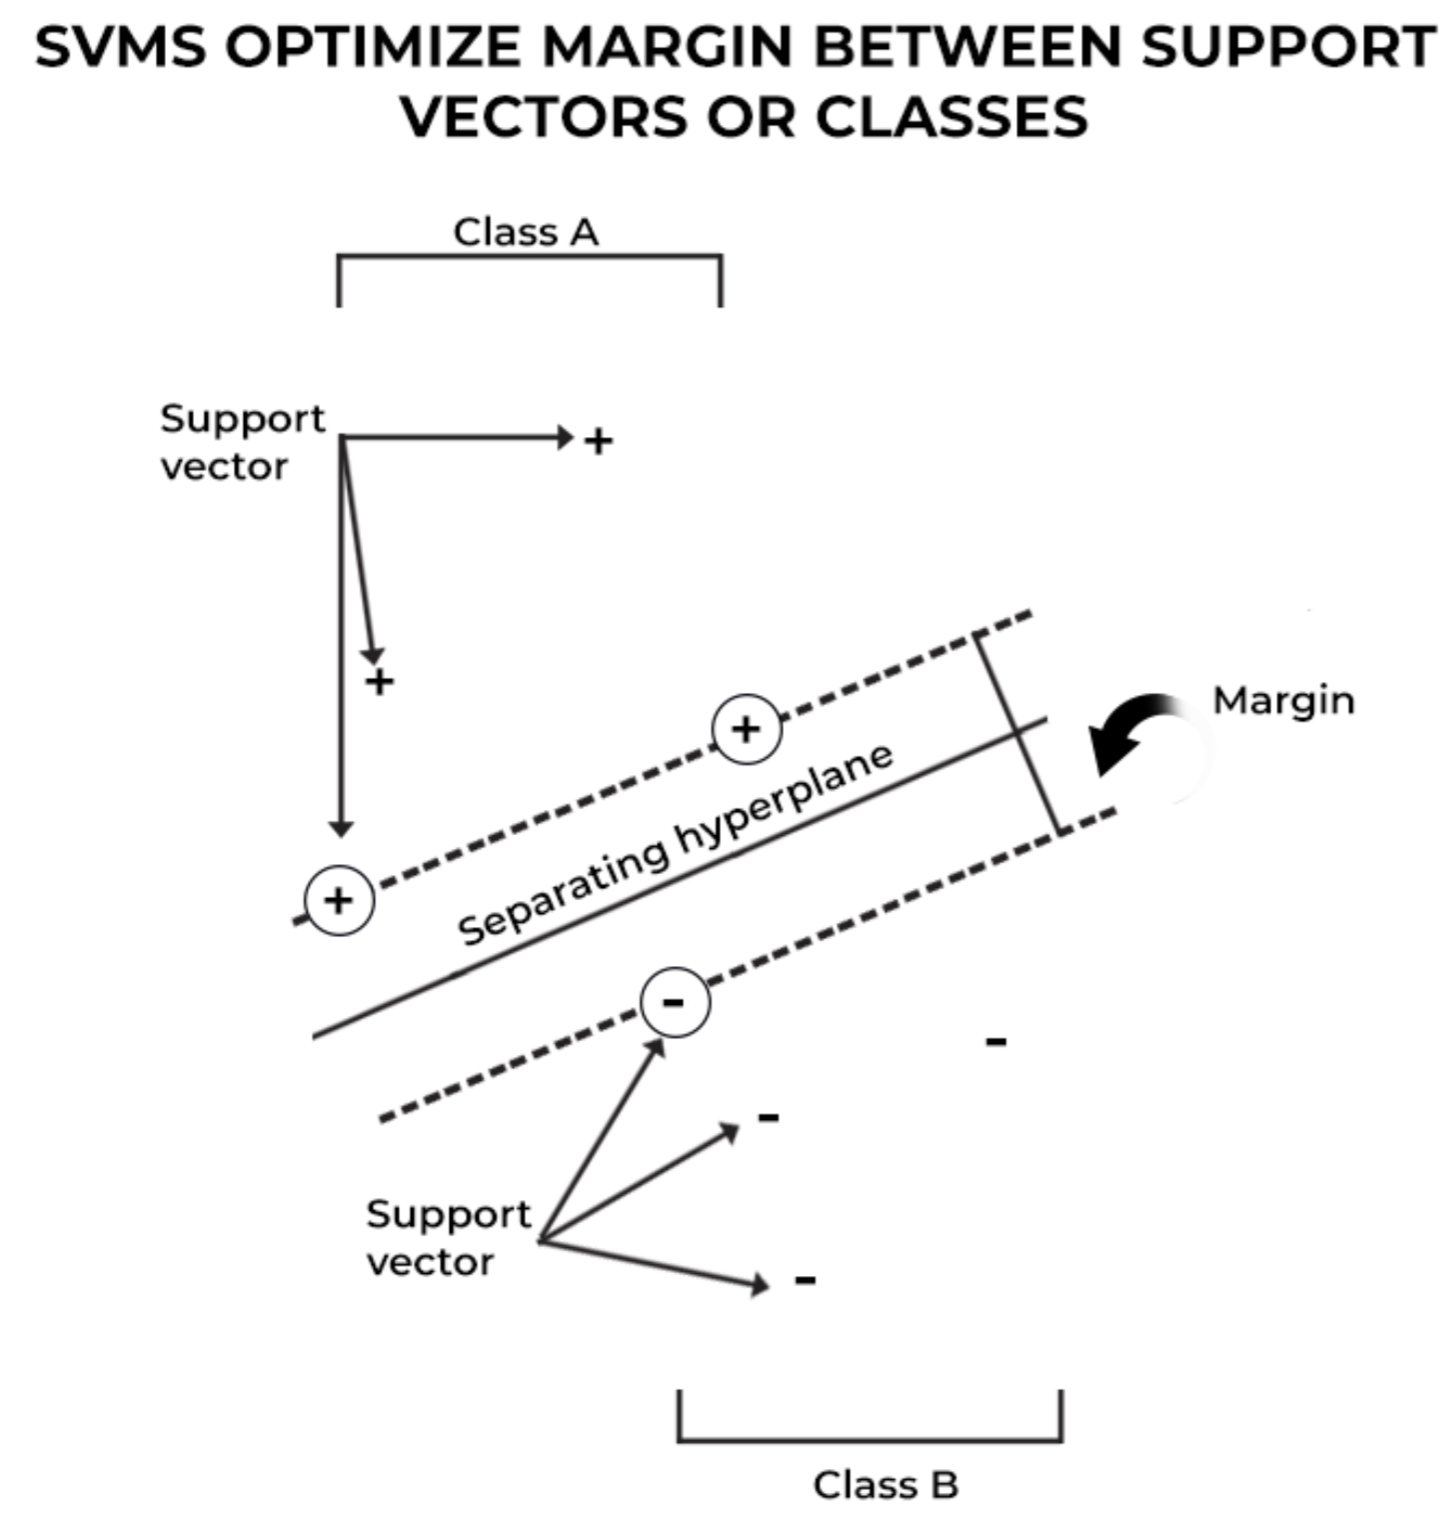
\includegraphics[width=8cm]{images/svm_b.png}
\end{center}
\caption{SVMs Optimize Margin Between Support Vectors or Classes}
\end{figure}
\\
\textbf{As seen in the above figure}, the margin refers to the maximum width of the slice that runs parallel to the hyperplane without any internal support vectors. Such hyperplanes are easier to define for linearly separable problems; however, for real-life problems or scenarios, the SVM algorithm tries to maximize the margin between the support vectors, thereby giving rise to incorrect classifications for smaller sections of data points.\\
\textbf{SVMs} are potentially designed for binary classification problems. However, with the rise in computationally intensive multiclass problems, several binary classifiers are constructed and combined to formulate SVMs that can implement such multiclass classifications through binary means. SVM works for classification:
\begin{enumerate}
\item \textbf{Data Representation:} The input data is represented as feature vectors in an n-dimensional space, where each dimension corresponds to a feature.
\item \textbf{Finding the Hyperplane:} SVM aims to find the hyperplane that maximizes the margin between the classes. The hyperplane is a decision boundary that separates the data points into different classes. In a binary classification scenario, this hyperplane is a line in 2D space, a plane in 3D space, and a hyperplane in higher-dimensional spaces.
\item \textbf{Maximizing Margin:} The margin is the distance between the hyperplane and the nearest data points from each class, known as support vectors. SVM aims to maximize this margin, as it generalizes better to unseen data and improves the classifier's robustness.
\item \textbf{Handling Non-Linearity:} In cases where the data is not linearly separable, SVM can still find a separating hyperplane by transforming the input space into a higher-dimensional space using a technique called the kernel trick. This allows SVM to effectively deal with non-linear decision boundaries.
\item \textbf{Classification:} Once the hyperplane is determined, classification of new data points is done by evaluating which side of the hyperplane they fall on. If a point lies on one side of the hyperplane, it's classified as belonging to one class; if it lies on the other side, it's classified as belonging to the other class.
\item \textbf{Optimization:} SVM involves solving an optimization problem to find the optimal hyperplane. The objective is to minimize the classification error while maximizing the margin. This is typically done using techniques such as gradient descent or quadratic programming.
\end{enumerate}

\textbf{SVMs} have several advantages, including their effectiveness in high-dimensional spaces, ability to handle non-linear decision boundaries, and resistance to overfitting. However, they can be sensitive to the choice of kernel and parameters, and they can be computationally expensive, especially with large datasets.

\subsubsection{Random Forest Regression}
\textbf{Random Forest Regression} is a supervised learning algorithm and bagging technique that uses an ensemble learning method for regression in machine learning. The trees in random forests run in parallel, meaning there is no interaction between these trees while building the trees.
\begin{figure}[h!]
\begin{center}
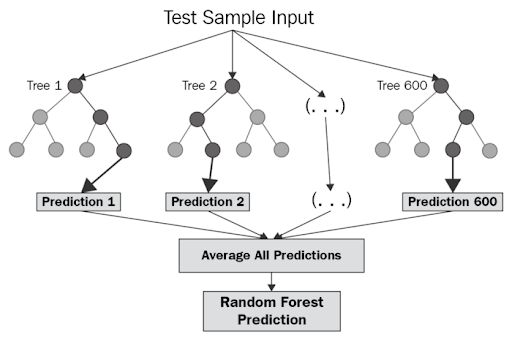
\includegraphics[width=8cm]{images/example1.jpg}
\end{center}
\caption{Random Forest sample}
\end{figure}

Random forest operates by constructing a multitude of decision trees at training time and outputting the class that’s the mode of the classes (classification) or mean prediction (regression) of the individual trees.
A random forest is a meta-estimator (i.e. it combines the result of multiple predictions), which aggregates many decision trees with some helpful modifications.\\
\\
\textbf{Advantages:}
\begin{enumerate}
    \item Random forest is one of the most accurate learning algorithms available. For many data sets, it produces a highly accurate classifier.
    \item It runs efficiently on large databases.
    \item It can handle thousands of input variables without variable deletion.
    \item It gives estimates of what variables are important in the classification.
    \item It generates an internal unbiased estimate of the generalization error as the forest building progresses.
    \item It has an effective method for estimating missing data and maintains accuracy when a large proportion of the data are missing.
\end{enumerate}

\subsubsection{Analysis of Variance}

Analysis of variance (ANOVA) is a statistical test used to evaluate the difference between the means of more than two groups. This statistical analysis tool separates the total variability within a data set into two components: random and systematic factors.
A one-way ANOVA uses one independent variable. A two-way ANOVA uses two independent variables. Analysts use the ANOVA test to determine independent variables' influence on the dependent variable in a regression study.
\\
\\
\textbf{Key Takeaways}
\begin{enumerate}
    \item Analysis of variance (ANOVA) is a statistical test used to evaluate the difference between the means of more than two groups.
    \item A one-way ANOVA uses one independent variable. A two-way ANOVA uses two independent variables.
    \item If no true variance exists between the groups, the ANOVA's F-ratio should equal close to 1.
\end{enumerate}
\textbf{Using ANOVA}
\begin{enumerate}
    \item An ANOVA test can be applied when data needs to be experimental. Analysis of variance is employed if there is no access to statistical software and ANOVA must be calculated by hand. It is simple to use and best suited for small samples. It is employed with subjects, test groups, and between and among groups.
    \item ANOVA is similar to multiple two-sample t-tests. However, it results in fewer type I errors. ANOVA groups differences by comparing each group's means and includes spreading the variance into diverse sources. Analysts use a one-way ANOVA with collected data about one independent variable and one dependent variable. A two-way ANOVA uses two independent variables. The independent variable should have at least three different groups or categories. ANOVA determines if the dependent variable changes according to the level of the independent variable. 

    \item A researcher might test students from multiple colleges to see if students from one of the colleges consistently outperform students from the other schools. In a business application, an R\&D researcher might test two different processes of creating a product to see if one is better than the other in terms of cost efficiency.
\end{enumerate}

\begin{equation*}
    F = \frac{MST}{MSE}
\end{equation*}
where:
\begin{itemize}
    \item $F$: ANOVA coefficient.
    \item $MST$: Mean sum of squares due to treatment.
    \item $MSE$: Mean sum of squares due to error.
\end{itemize}





\textbf{One-Way vs. Two-Way ANOVA}
\begin{enumerate}
    \item A one-way ANOVA evaluates the impact of a sole factor on a sole response variable. It determines whether all the samples are the same. The one-way ANOVA is used to determine whether there are any statistically significant differences between the means of three or more independent groups.

    \item A two-way ANOVA is an extension of the one-way ANOVA. With a one-way, you have one independent variable affecting a dependent variable. With a two-way ANOVA, there are two independents. For example, a two-way ANOVA allows a company to compare worker productivity based on two independent variables, such as salary and skill set. It is utilized to observe the interaction between the two factors and test the effect of two factors simultaneously.
\end{enumerate}
\subsubsection{Welch’s Test}
Welch’s Test for Unequal Variances (also called Welch’s t test, Welch’s adjusted T or unequal variances t-test) is a modification of Student’s t-test(more reliable when the two samples have unequal variances and/or unequal sample sizes) to see if two sample means are significantly different. The modification is to the degrees of freedom used in the test, which increases the test power for samples with unequal variance. There are two hypotheses in the Welch’s test:

\begin{itemize}
    \item Null hypothesis $H_0$: for the test is that the means are equal.
    \item Alternative hypothesis $H_1$: for the test is that means are not equal.
\end{itemize}
Below is the formula of Welch’s test:
\begin{equation*}
    t = \dfrac{\overline{X_1}-\overline{X_2}}{\sqrt{\dfrac{s^2_1}{n_1}+\dfrac{s^2_2}{n_2}}}=\dfrac{\overline{X_1}-\overline{X_2}}{\sqrt{se^2_1+se^2_2}}
\end{equation*}
where:
\begin{itemize}
    \item $\overline{X_i}$ is the $i^{th}$ sample mean.
    \item $s_i$ is the $i^{th}$ standard deviation.
\end{itemize}
\pagebreak
\section{Descriptive statistics}
\subsection{Data Preprocessing}
\subsubsection{Import and Selection}
\begin{mdframed}[leftline=false,rightline=false,backgroundcolor=lightblue!10,nobreak=false]
    \begin{minted}[linenos,breaklines,breaksymbolleft=,obeytabs=true,tabsize=2]{R}
pacman::p_load(
  dplyr,   #data manipulation
  ggplot2, #visualization
  ggfortify, #visualization
  ggcorrplot, #statistical modeling
  broom, #additional visualization functionalities
  rio # for export function
)
all_gpus <- read.csv("All_GPUs.csv")
data = all_gpus %>% select("Manufacturer","Boost_Clock","Core_Speed","Max_Power","Memory",
"Memory_Bandwidth","Memory_Bus","Memory_Speed","Release_Price","Shader","TMUs")
    \end{minted}
\end{mdframed}
- After review, our team chose to extract 11 out of 34 variables: \textbf{Manufacturer, Boost\textunderscore Clock, Core\textunderscore Speed, Max\textunderscore Power, Memory, Memory\textunderscore Bandwidth, Memory\textunderscore Bus, Memory\textunderscore Speed, Release\textunderscore Price, Shader, TMUs.}\\
- This is the summary of the chosen data:
\lstinputlisting[language={},numbers=none,caption={Summary}]{txt/1.txt}
\subsubsection{Conversion}
Since some of the attributes are \textbf{character}, we will convert it to number using function $as.numeric(...)$. After conversion, here is the result:
\lstinputlisting[language={},numbers=none,caption={5 lines of data after conversion}]{txt/2.txt}
After choosing the appropriate attributes and converting them to reproducible types (numeric), we now have the subset of the original raw dataset. However, we should check missing values using function $colSums(is.na(data))$. Here is the result:
\lstinputlisting[language={},numbers=none,caption={Missing values}]{txt/3.txt}
\subsubsection{Applying k-NN to the dataset}
In order to \textbf{deal with missing values}, our team used \textbf{K-Nearest Neighbor model} as introduced in the background to predict the missing values. When applying model to the dataset, we choose k (numbers of nearest neighbors used) equals to square root of numbers of observations (3406) \textbf{(kNN(data, k = sqrt(nrow(data)), imp\textunderscore var = FALSE))}. Here is the view of dataset:
\begin{figure}[h!]
\begin{center}
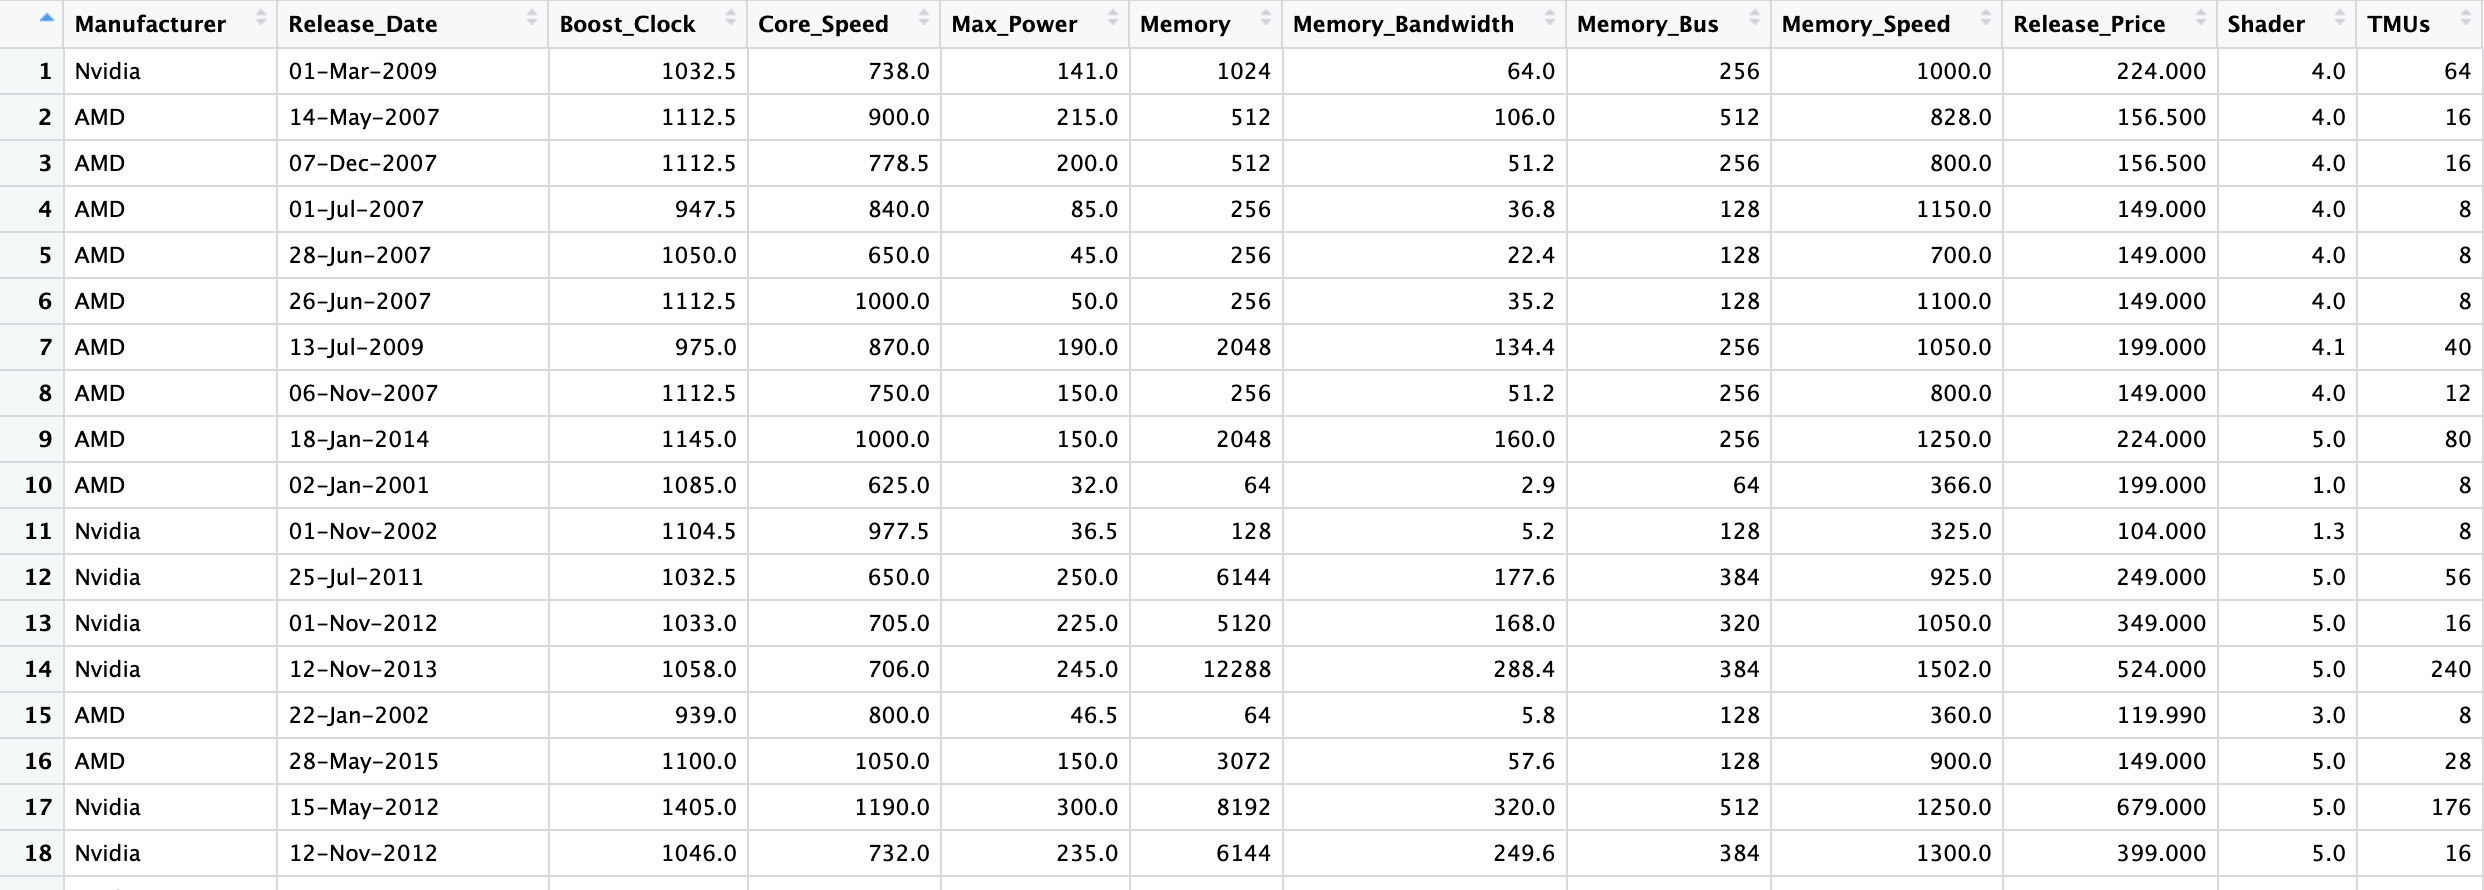
\includegraphics[width=16cm]{images/1.png}
\end{center}
\caption{View of dataset after k-NN}
\end{figure}
\\
For later use, we export the dataset to \textbf{"gpu\textunderscore clean.csv"} file.
\begin{mdframed}[leftline=false,rightline=false,backgroundcolor=lightblue!10,nobreak=false]
    \begin{minted}[linenos,breaklines,breaksymbolleft=,obeytabs=true,tabsize=2]{R}
export(df,"gpu_clean.csv") #for later_use
    \end{minted}
\end{mdframed}
\textbf{The reason we choose k-NN} is because this algorithm can compete with the most accurate model as it gives highly accurate predictions. The k-NN algorithm is a type of lazy learning, where the computation for the generation of the predictions is deferred until classification. Although this method increases the costs of computation compared to other algorithms, k-NN is still the better choice for applications where predictions are not requested frequently but where accuracy is important.
\subsection{Descriptive statistic}
\subsubsection{Summary}
After cleaning process, we certainly have a clear and clean dataset in the data frame with 0 missing value. Here is the summary of \textbf{df}:
\lstinputlisting[language={},numbers=none,caption={Summary of df}]{txt/4.txt}
Because \textbf{Manufacturer} and \textbf{Release\textunderscore Year} are categorical variables, we can not have an overview information in this variable, so we try to make these more specific:
\lstinputlisting[language={},numbers=none,caption={Summary of df}]{txt/5.txt}
\subsubsection{Plot}
Next, we take a better look at the distribution of the 10 independent variables, utilizing the Histogram and Boxplot:
\begin{center}
\begin{adjustbox}{width=\textwidth}
    \begin{tabular}{cc}
        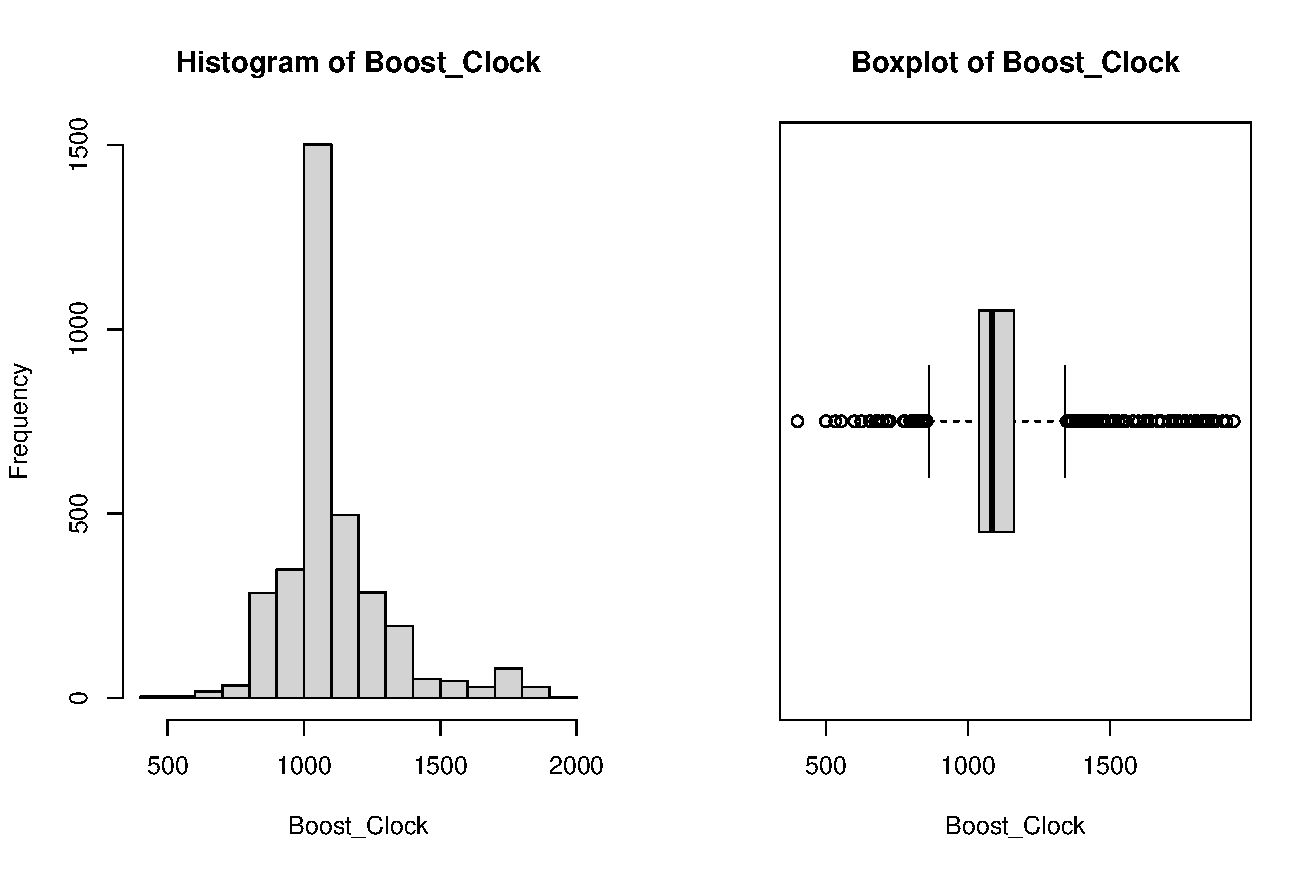
\includegraphics[keepaspectratio, width=1\textwidth, height=1\textheight]{Visualization/Rplot_1.pdf}
        &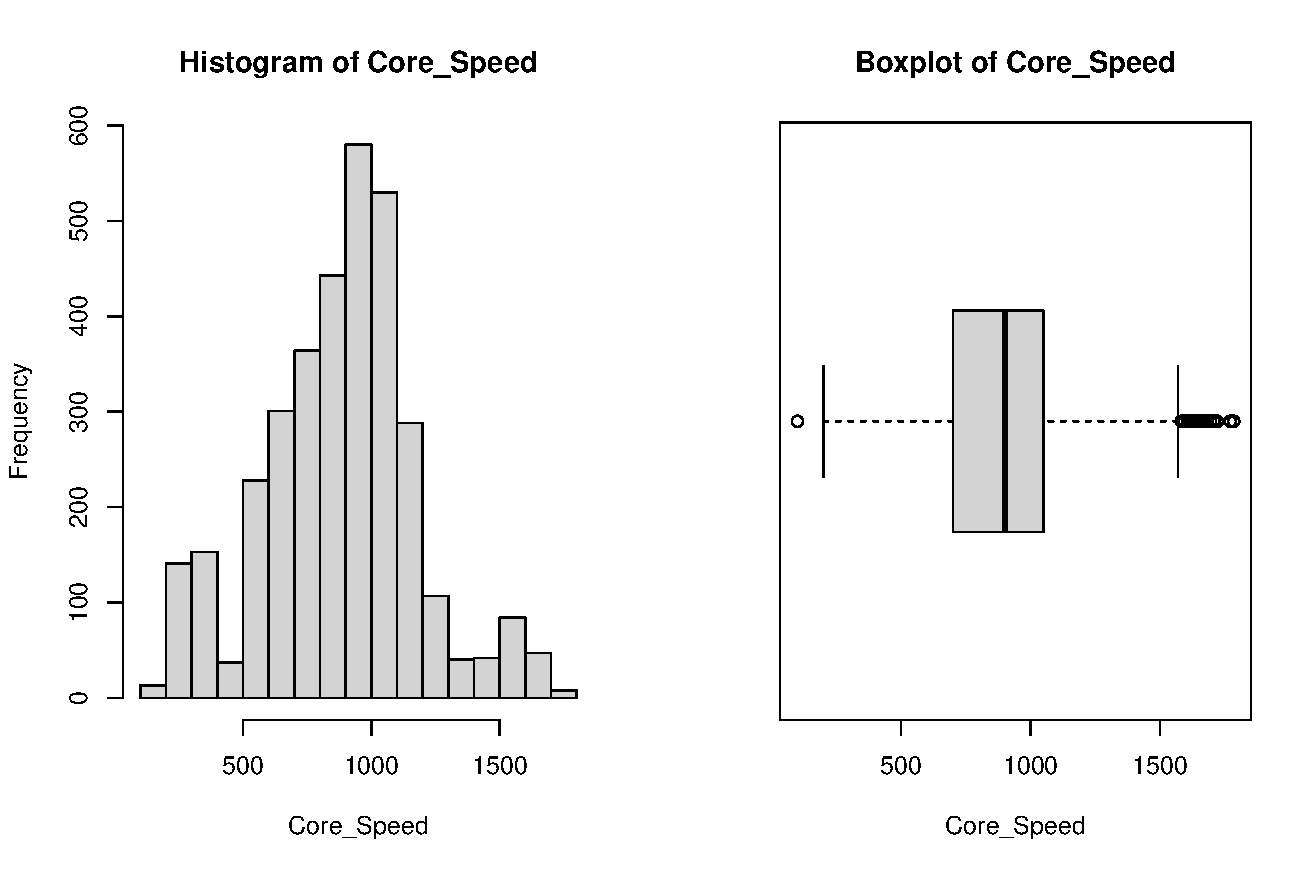
\includegraphics[keepaspectratio, width=1\textwidth, height=1\textheight]{Visualization/Rplot_2.pdf}\\
    \end{tabular}
\end{adjustbox}
\end{center}
\begin{center}
\begin{adjustbox}{width=\textwidth}
    \begin{tabular}{cc}
        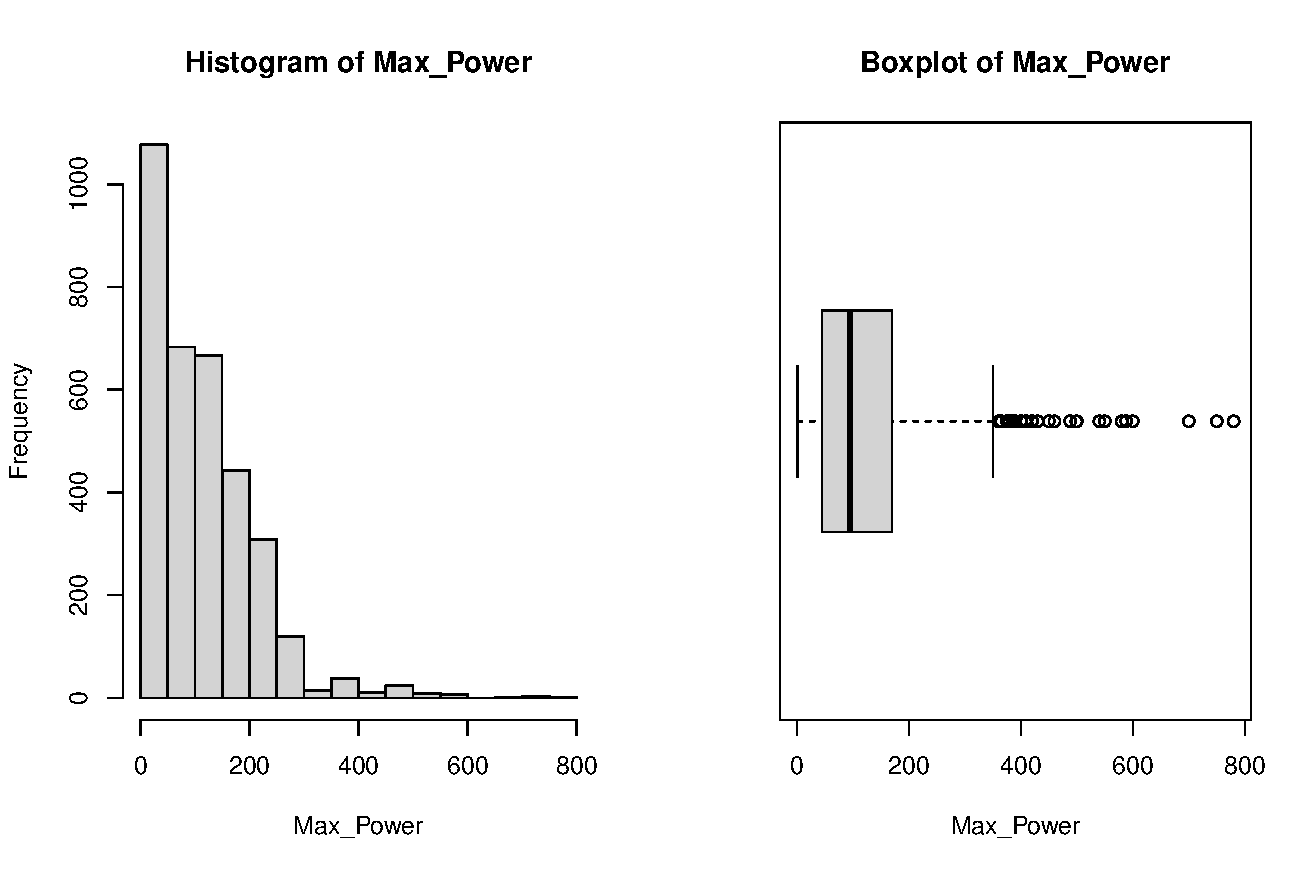
\includegraphics[keepaspectratio, width=1\textwidth, height=1\textheight]{Visualization/Rplot_3.pdf}
        &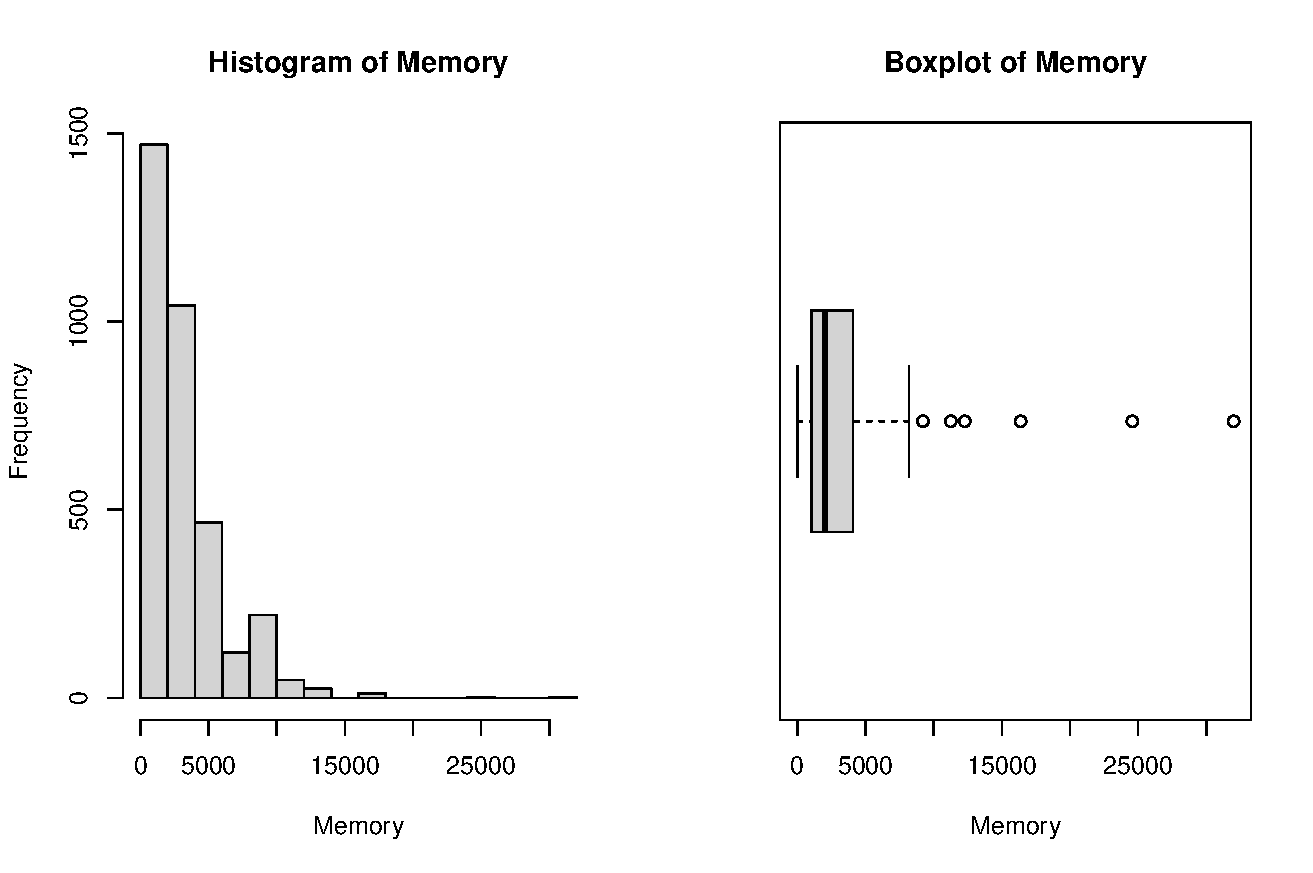
\includegraphics[keepaspectratio, width=1\textwidth, height=1\textheight]{Visualization/Rplot_4.pdf}\\
        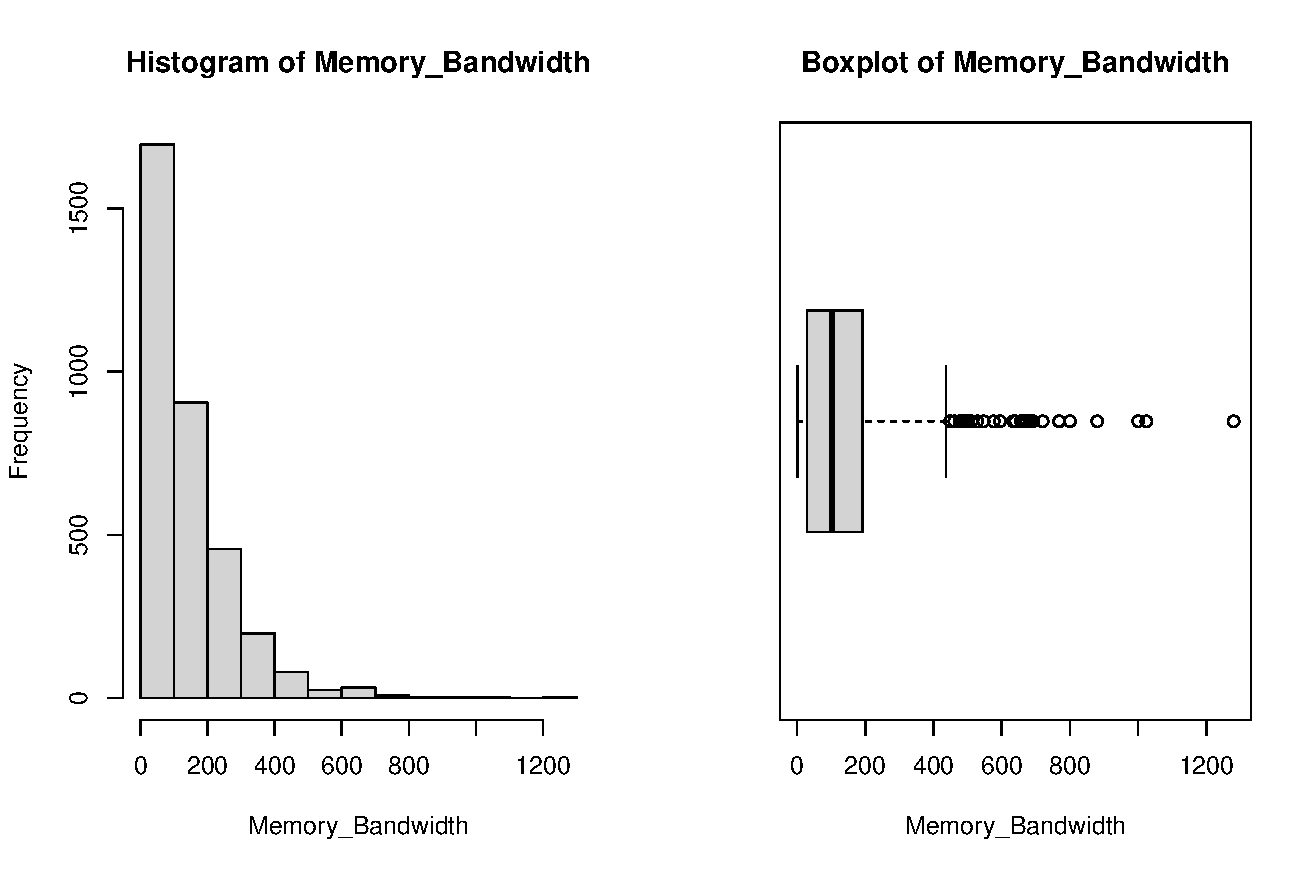
\includegraphics[keepaspectratio, width=1\textwidth, height=1\textheight]{Visualization/Rplot_5.pdf}
        &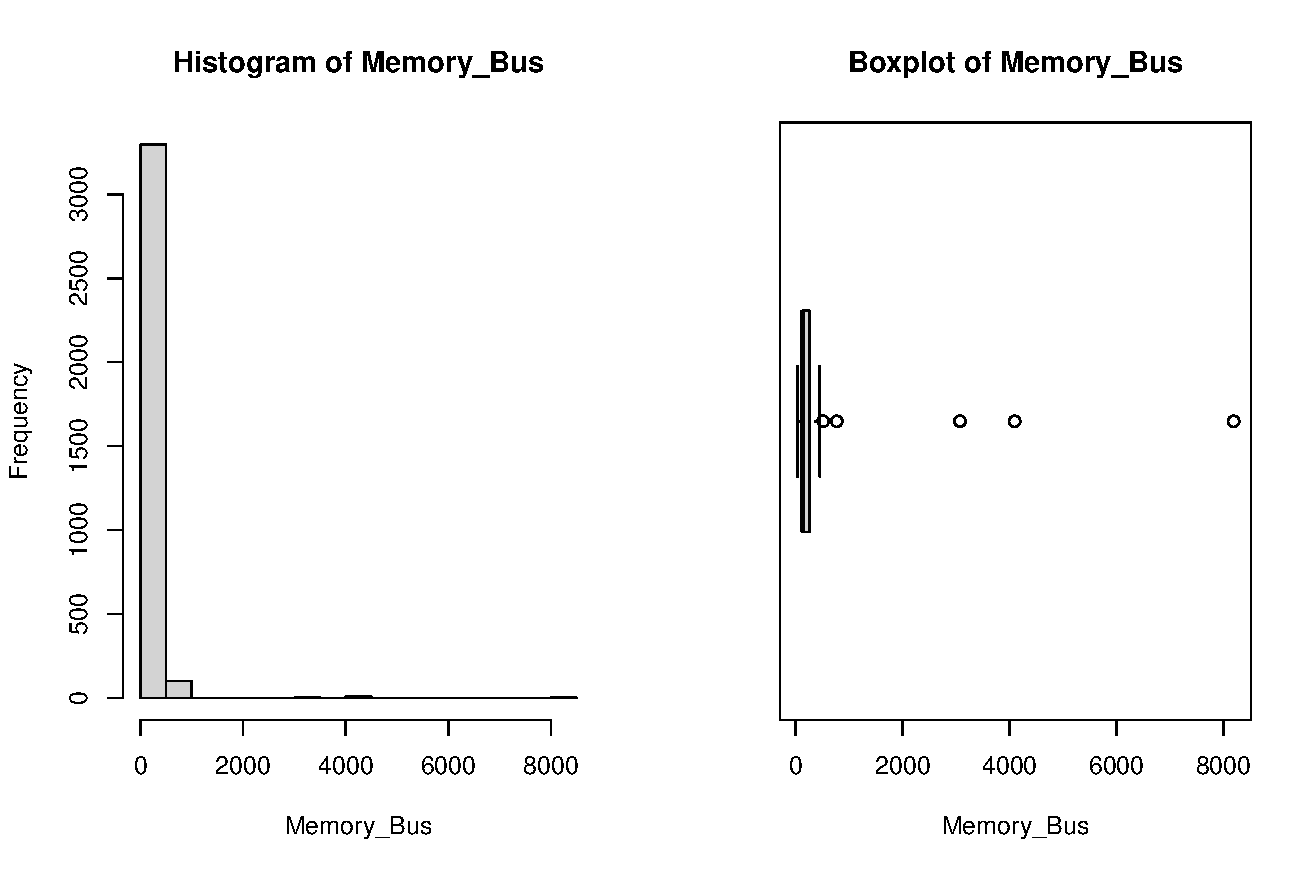
\includegraphics[keepaspectratio, width=1\textwidth, height=1\textheight]{Visualization/Rplot_6.pdf}\\
        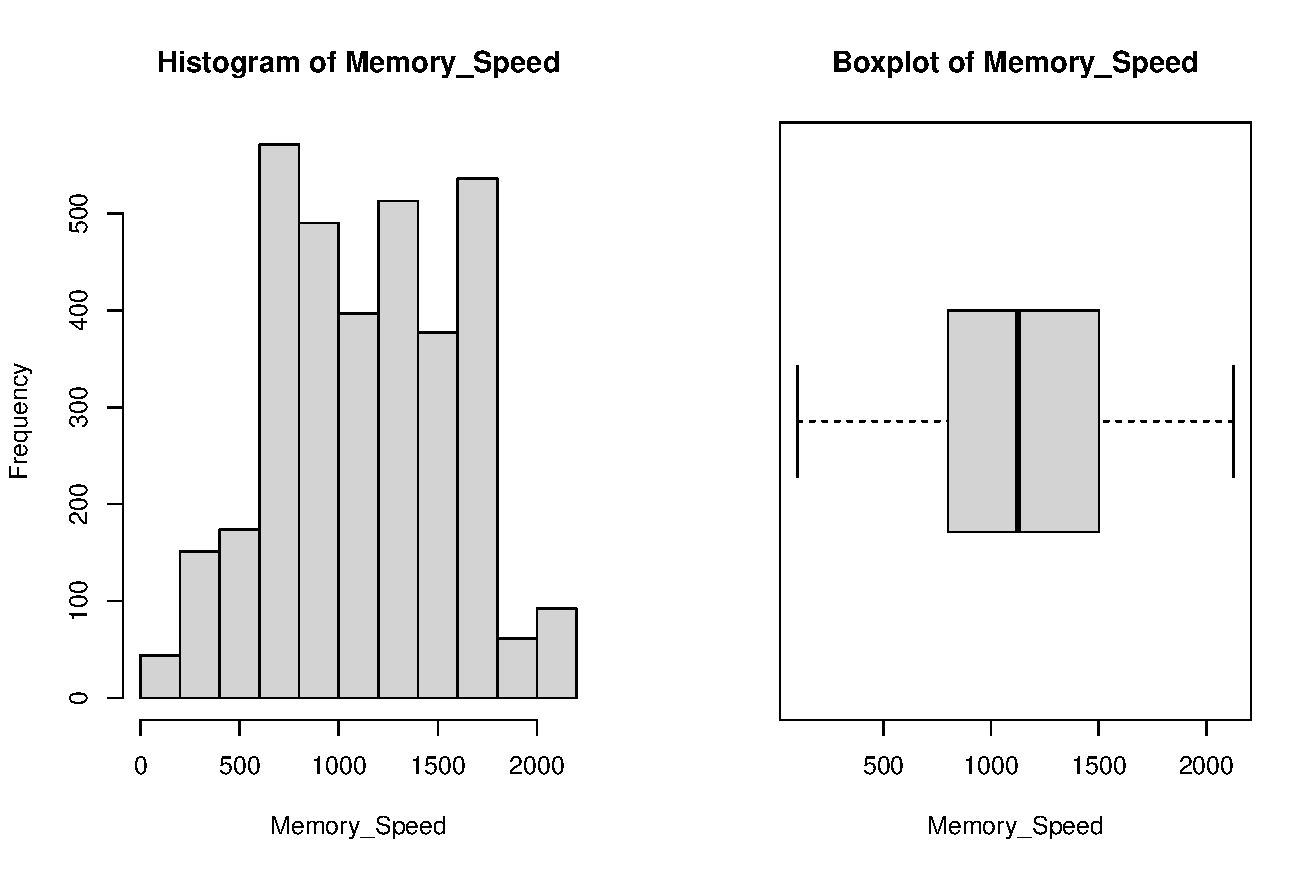
\includegraphics[keepaspectratio, width=1\textwidth, height=1\textheight]{Visualization/Rplot_7.pdf}
        &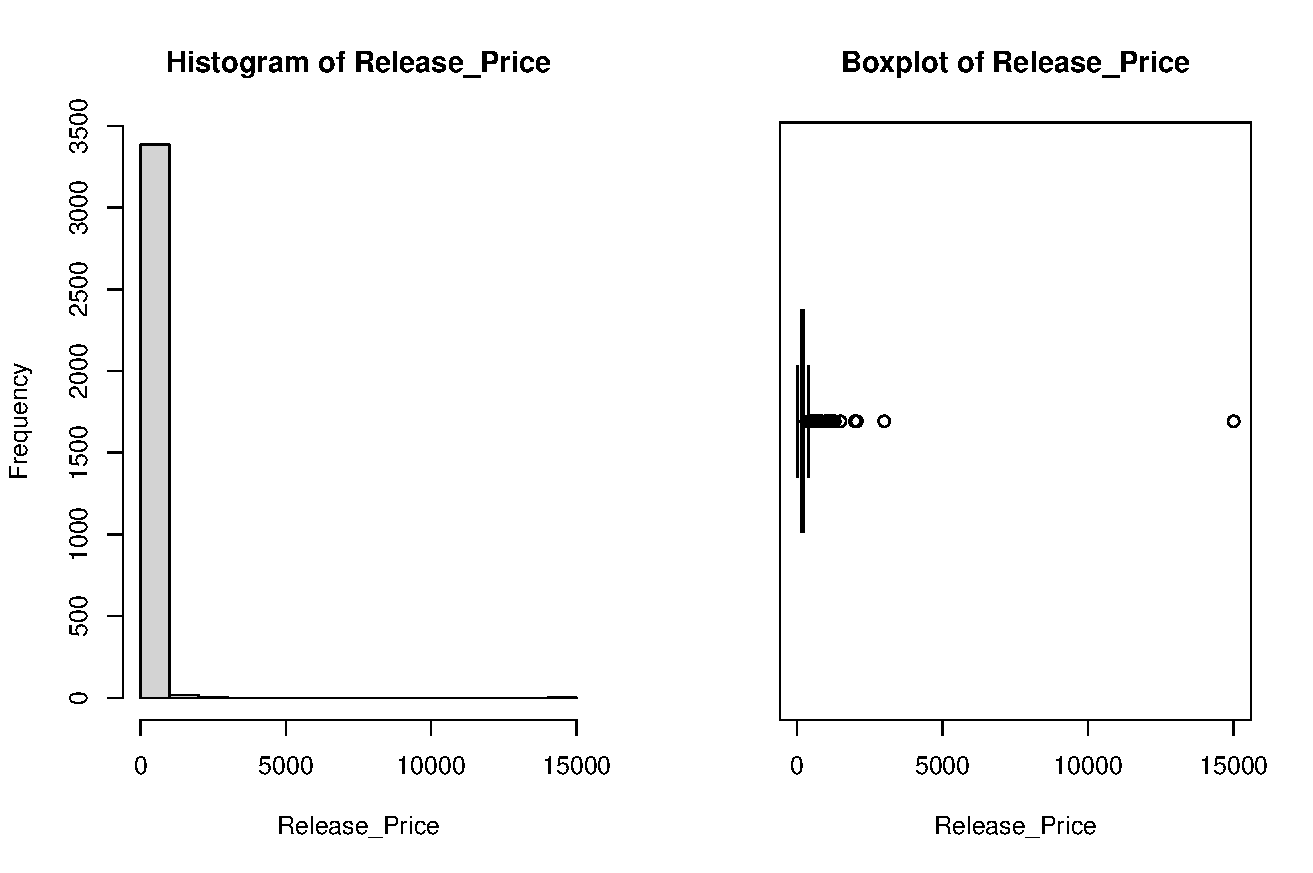
\includegraphics[keepaspectratio, width=1\textwidth, height=1\textheight]{Visualization/Rplot_8.pdf}\\
    \end{tabular}
\end{adjustbox}
\end{center}
\begin{center}
\begin{adjustbox}{width=\textwidth}
    \begin{tabular}{cc}
        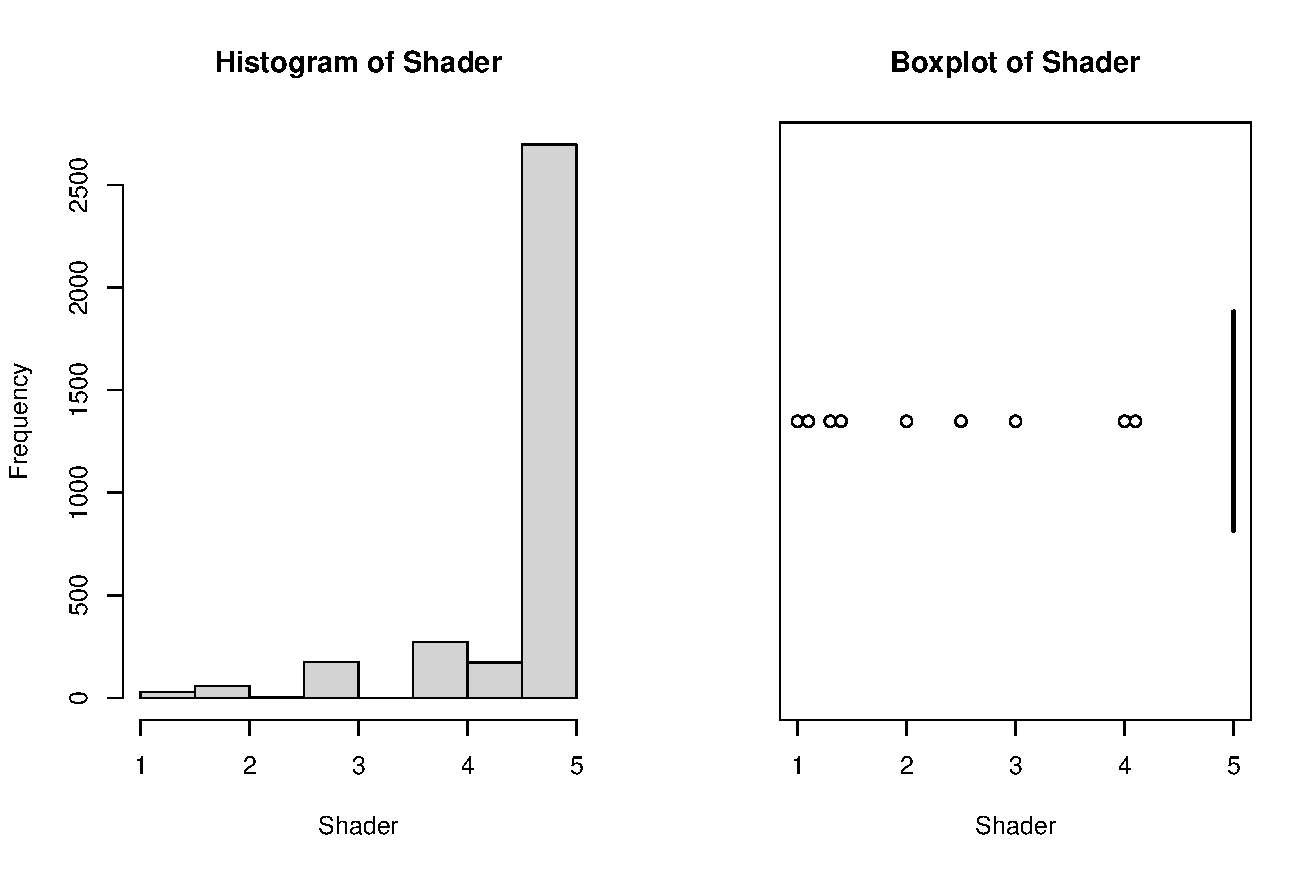
\includegraphics[keepaspectratio, width=1\textwidth, height=1\textheight]{Visualization/Rplot_9.pdf}
        &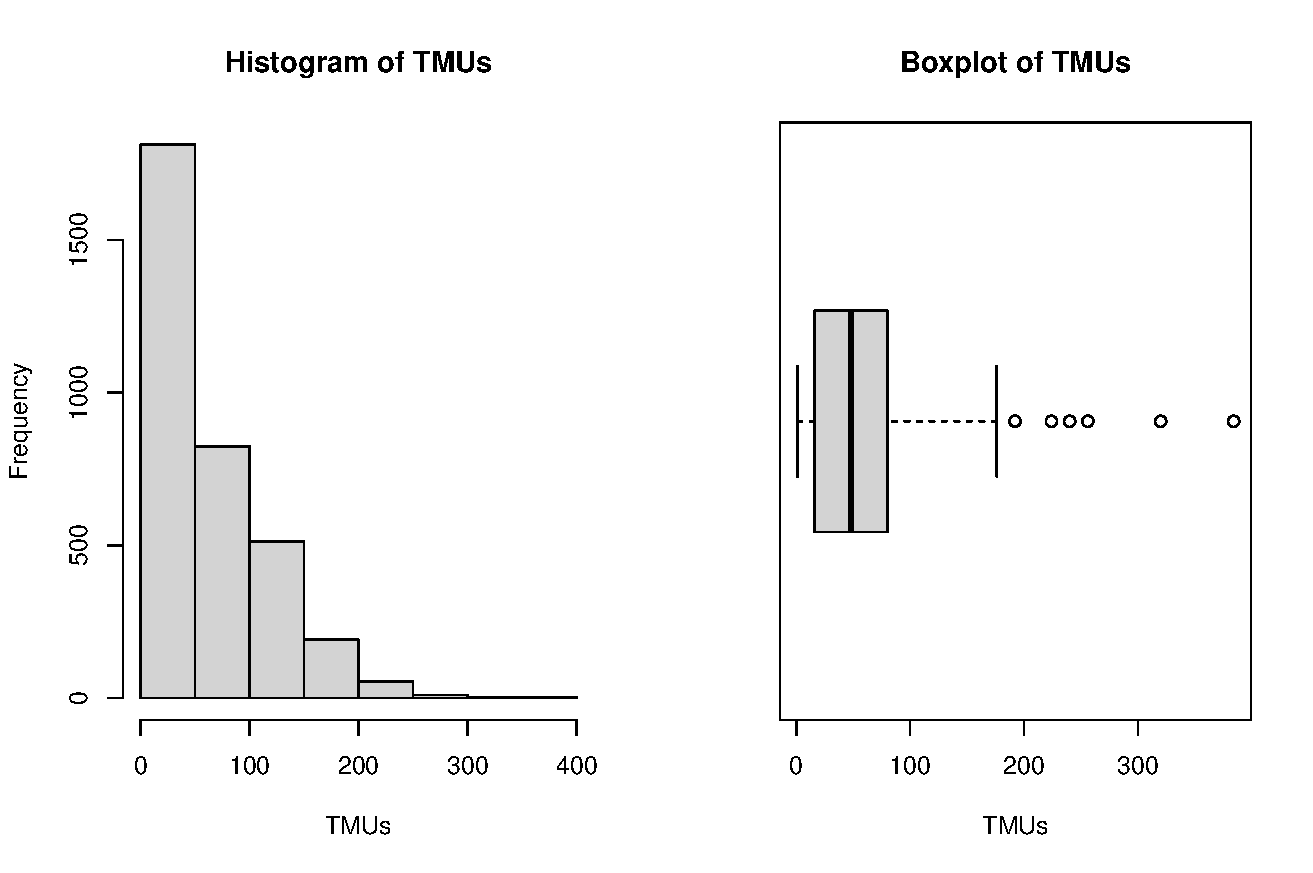
\includegraphics[keepaspectratio, width=1\textwidth, height=1\textheight]{Visualization/Rplot_10.pdf}\\
    \end{tabular}
\end{adjustbox}
\end{center}
\textbf{Explanation: }
\begin{itemize}
    \item \verb|Boost Clock and Core Speed:|Both show distributions centered around 1000 MHz, with Boost Clock being slightly right-skewed and Core Speed more symmetric. Boxplots indicate medians around 1000 MHz with outliers on both ends, suggesting variations in clock speeds among different GPU models.
    \item \verb|Max Power:|Right-skewed distribution with most values under 200 Watts. Boxplot shows a median below 200 Watts, with outliers indicating higher power requirements for some GPUs.
    \item \verb|Memory:|Right-skewed distribution with most GPUs having up to 5000 MB. Boxplot median around 5000 MB, with outliers showing higher memory capacities.
    \item \verb|Memory Bandwidth and Memory Bus:|Both attributes show right-skewed distributions, indicating most GPUs have lower bandwidth and bus widths. Boxplots reveal medians at lower ranges with outliers suggesting higher specifications in some models.
    \item \verb|Memory Speed:|Multi-modal distribution, indicating common speeds at several points. Boxplot shows a median around 1000 units, with a symmetrical spread and outliers.
    \item \verb|Release Price:|Right-skewed distribution, most GPUs priced under 5000 units. Boxplot median around 5000 units, with some GPUs being significantly more expensive.
    \item \verb|Shader:|Highly skewed towards level 5, indicating a common standard or preference for this shader level in GPUs. Boxplot collapses at level 5, showing no variability among most GPUs and treating other levels as outliers.
    \item \verb|TMUs:|Right-skewed distribution, with most GPUs having fewer than 100 TMUs. Boxplot shows a median around 50 TMUs, with an interquartile range from about 25 to 75 TMUs and several outliers indicating higher performance models.
\end{itemize}
As can be seen, the attribute we considered (Release\textunderscore Price) is right-skewed, which is difficult for inferential statistics. So we will apply \textbf{log-transformation} to the dataset for a better representation.
\begin{mdframed}[leftline=false,rightline=false,backgroundcolor=lightblue!10,nobreak=false]
    \begin{minted}[linenos,breaklines,breaksymbolleft=,obeytabs=true,tabsize=2]{R}
df['Max_Power'] <- log(df['Max_Power'])
df['Boost_Clock'] <- log(df['Boost_Clock'])
df['Core_Speed'] <- log(df['Core_Speed'])
df['Memory'] <- log(df['Memory'])
df['Memory_Bandwidth'] <- log(df['Memory_Bandwidth'])
df['Memory_Bus'] <- log(df['Memory_Bus'])
df['Memory_Speed'] <- log(df['Memory_Speed'])
df['Release_Price'] <- log(df['Release_Price'])
df['Shader'] <- log(df['Shader'])
df['TMUs'] <- log(df['TMUs'])
    \end{minted}
\end{mdframed}
\begin{center}
\begin{adjustbox}{width=\textwidth}
    \begin{tabular}{cc}
        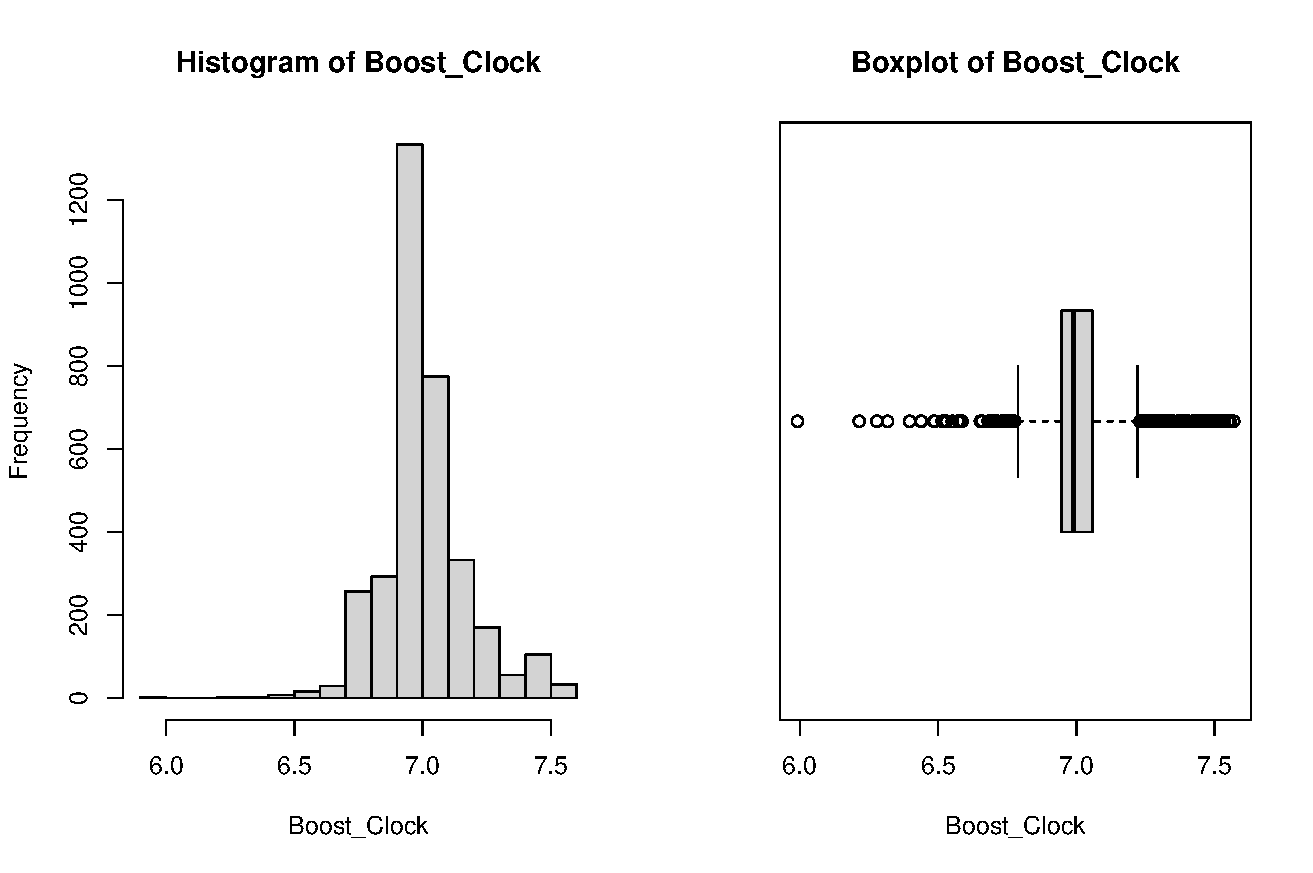
\includegraphics[keepaspectratio, width=1\textwidth, height=1\textheight]{Visualization/Rplot_11.pdf}
        &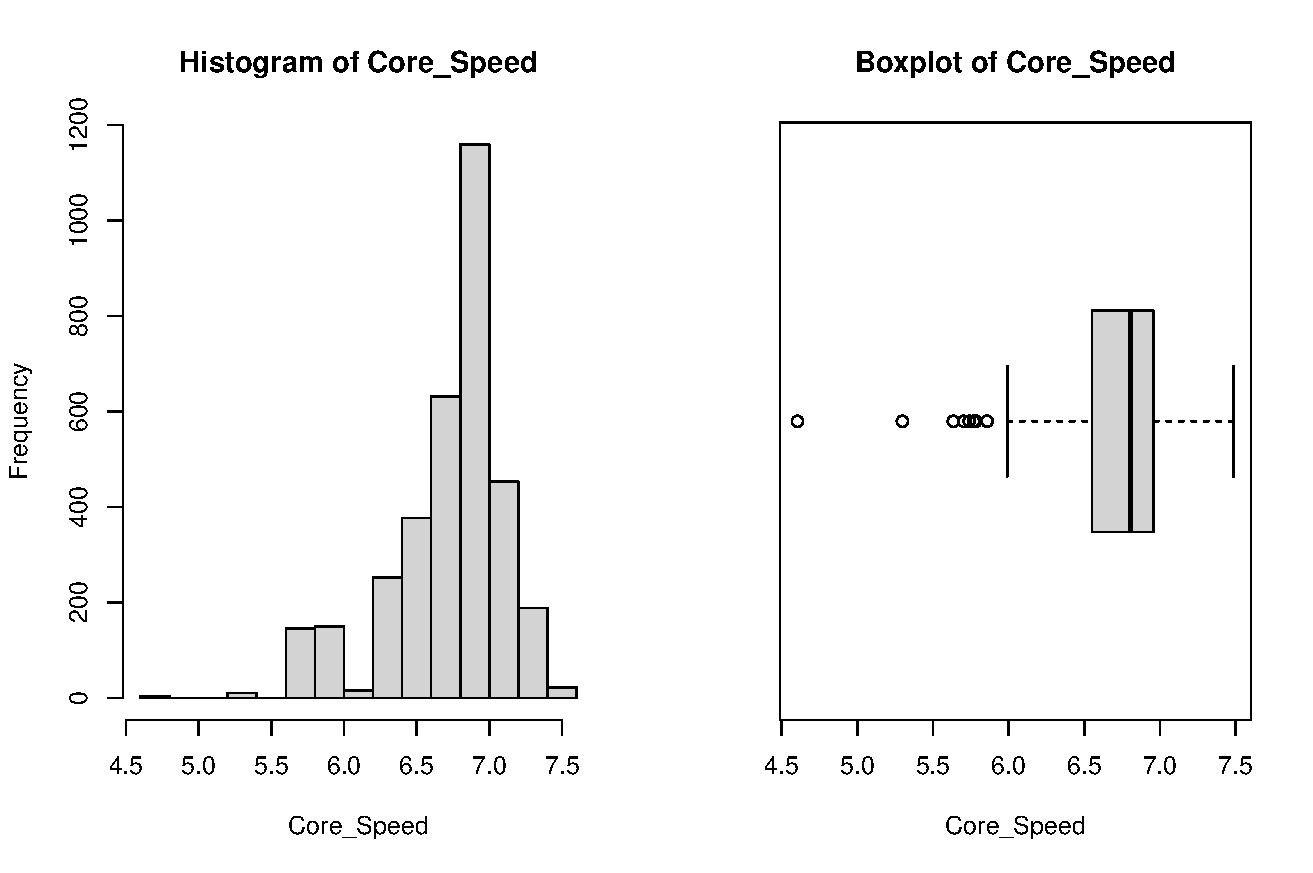
\includegraphics[keepaspectratio, width=1\textwidth, height=1\textheight]{Visualization/Rplot_12.pdf}\\
    \end{tabular}
\end{adjustbox}
\end{center}
\begin{center}
\begin{adjustbox}{width=\textwidth}
    \begin{tabular}{cc}
        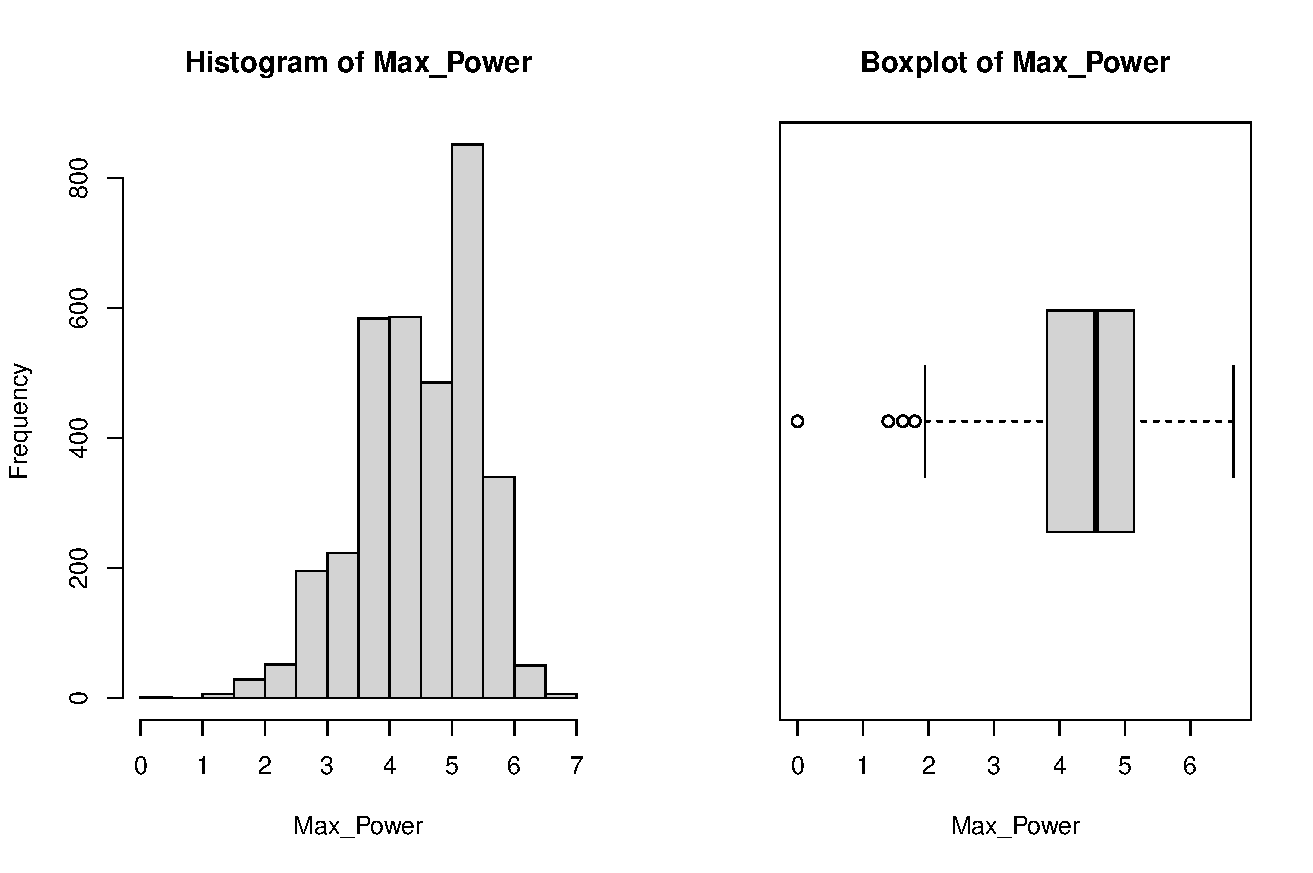
\includegraphics[keepaspectratio, width=1\textwidth, height=1\textheight]{Visualization/Rplot_13.pdf}
        &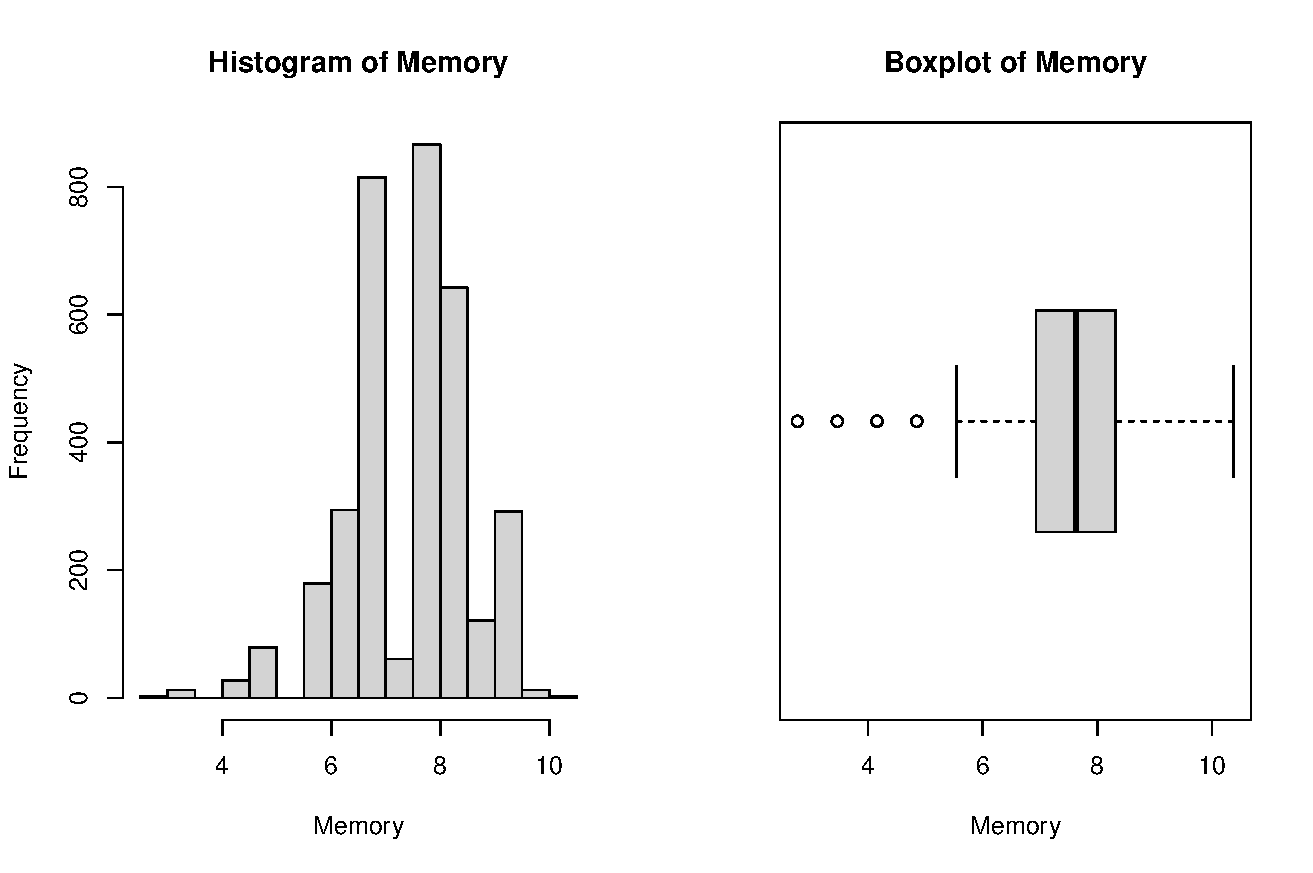
\includegraphics[keepaspectratio, width=1\textwidth, height=1\textheight]{Visualization/Rplot_14.pdf}\\
        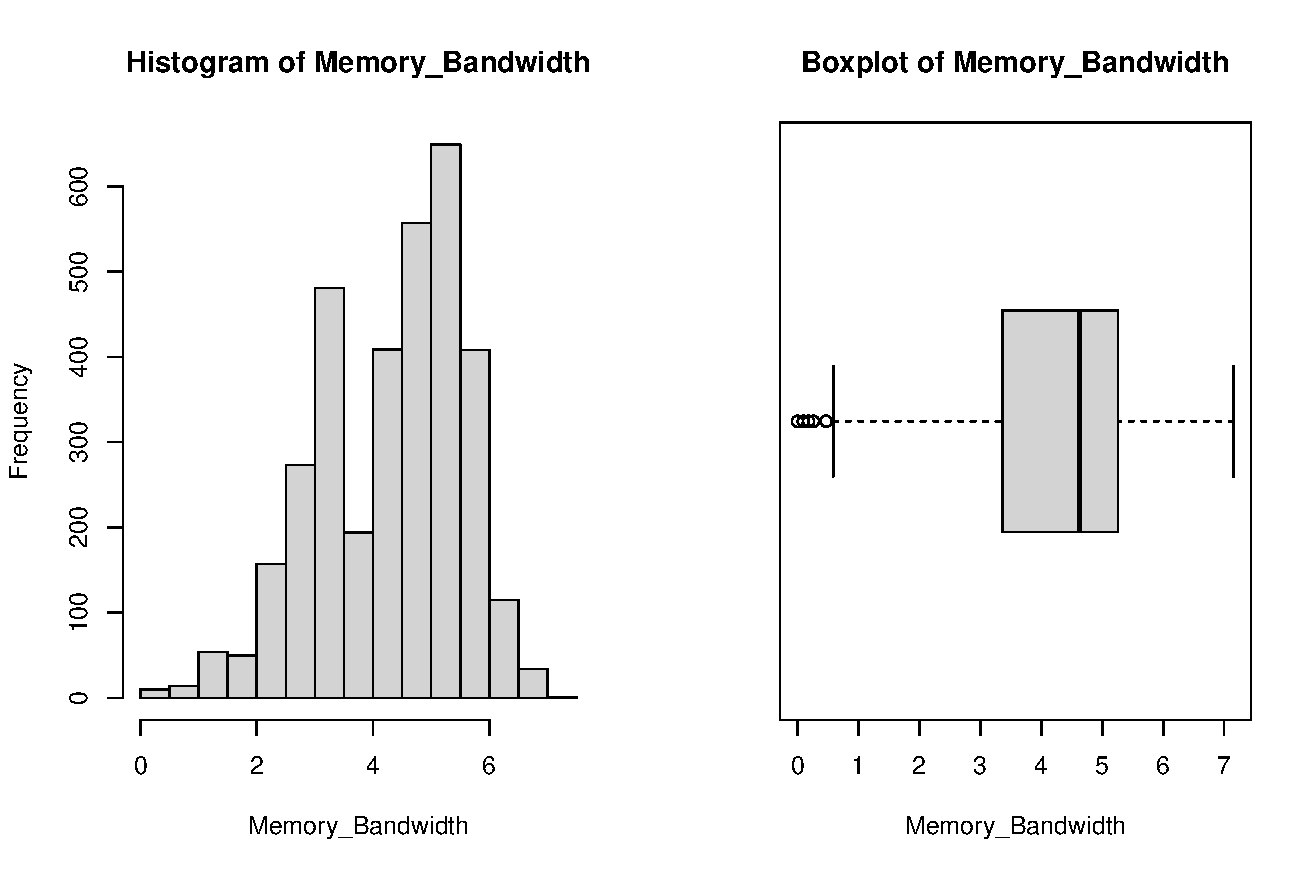
\includegraphics[keepaspectratio, width=1\textwidth, height=1\textheight]{Visualization/Rplot_15.pdf}
        &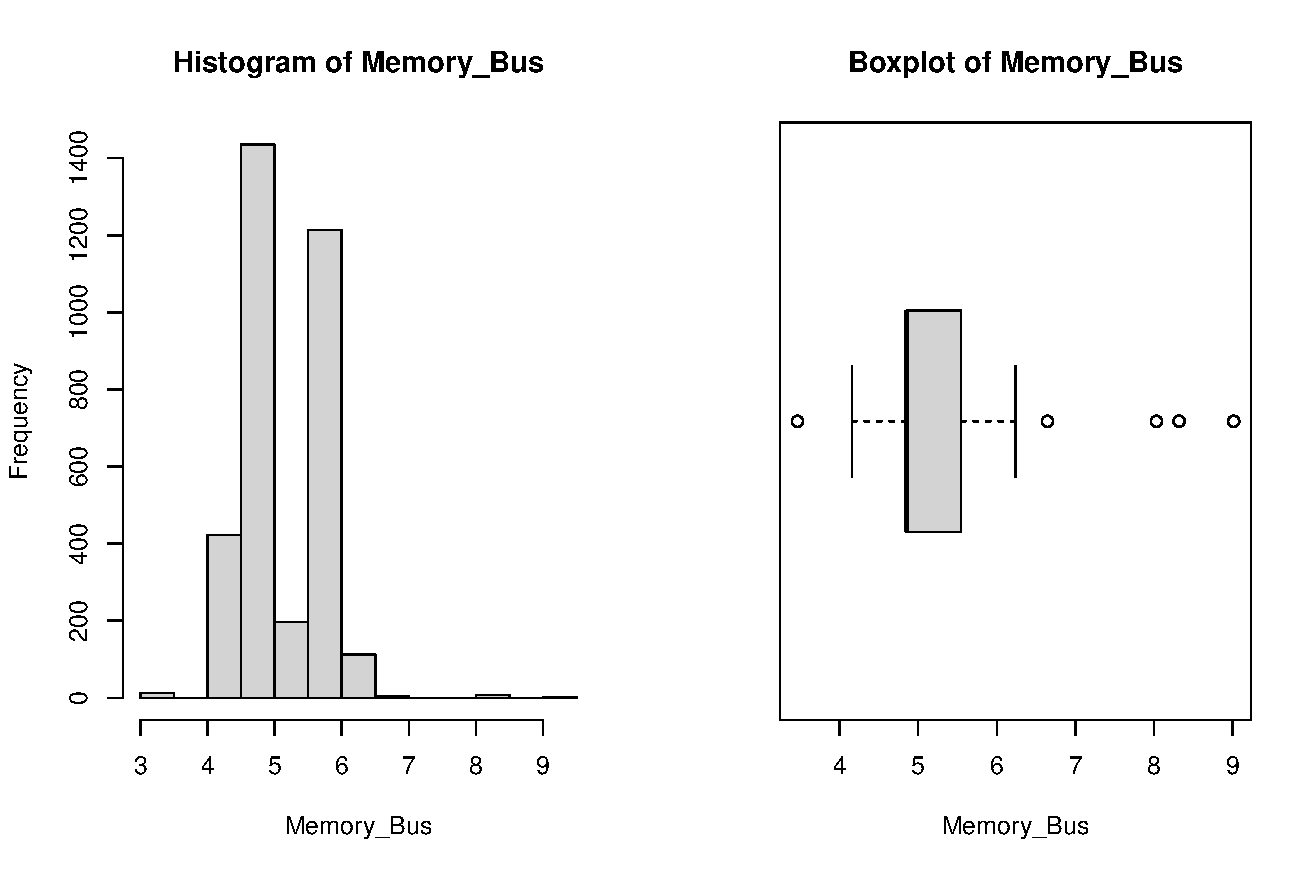
\includegraphics[keepaspectratio, width=1\textwidth, height=1\textheight]{Visualization/Rplot_16.pdf}\\
        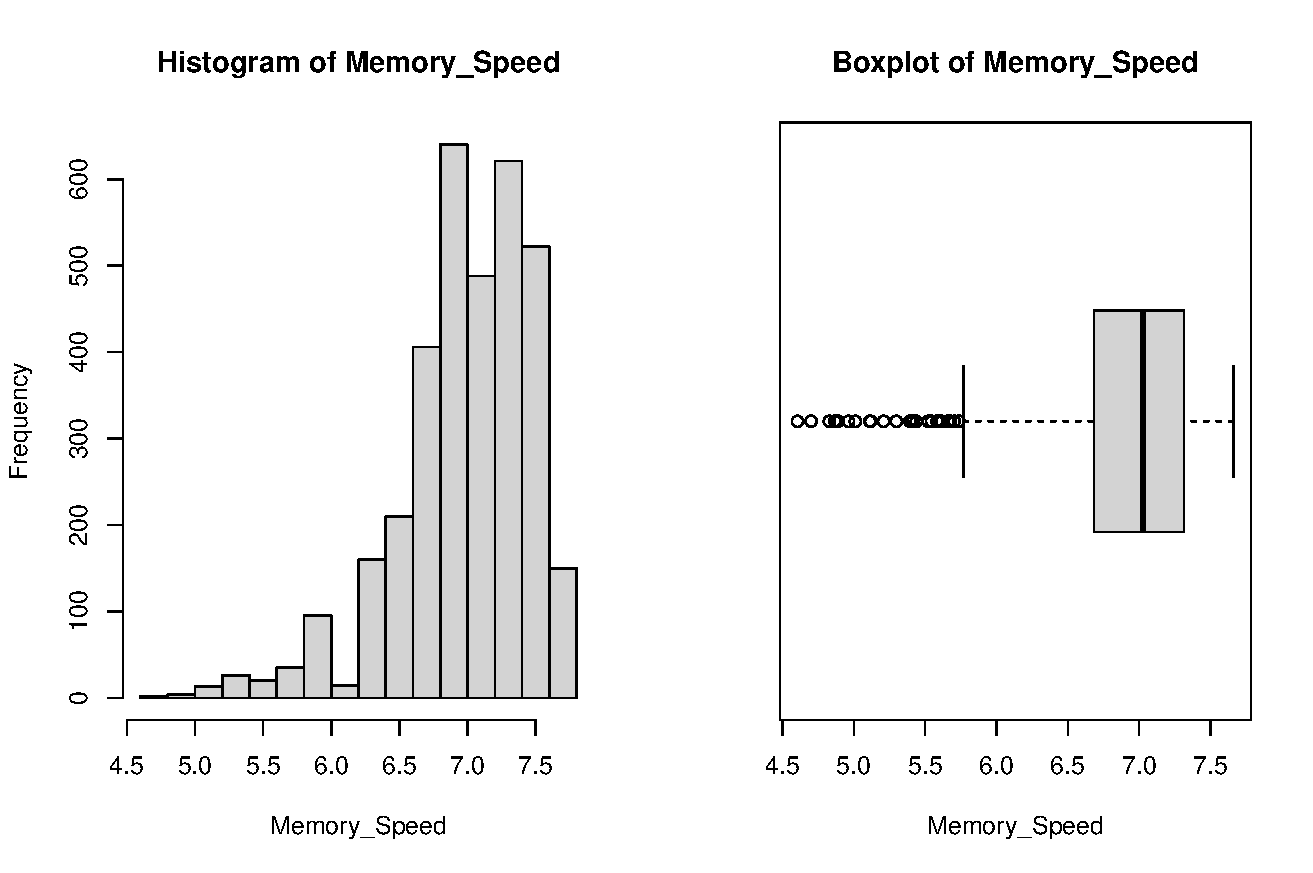
\includegraphics[keepaspectratio, width=1\textwidth, height=1\textheight]{Visualization/Rplot_17.pdf}
        &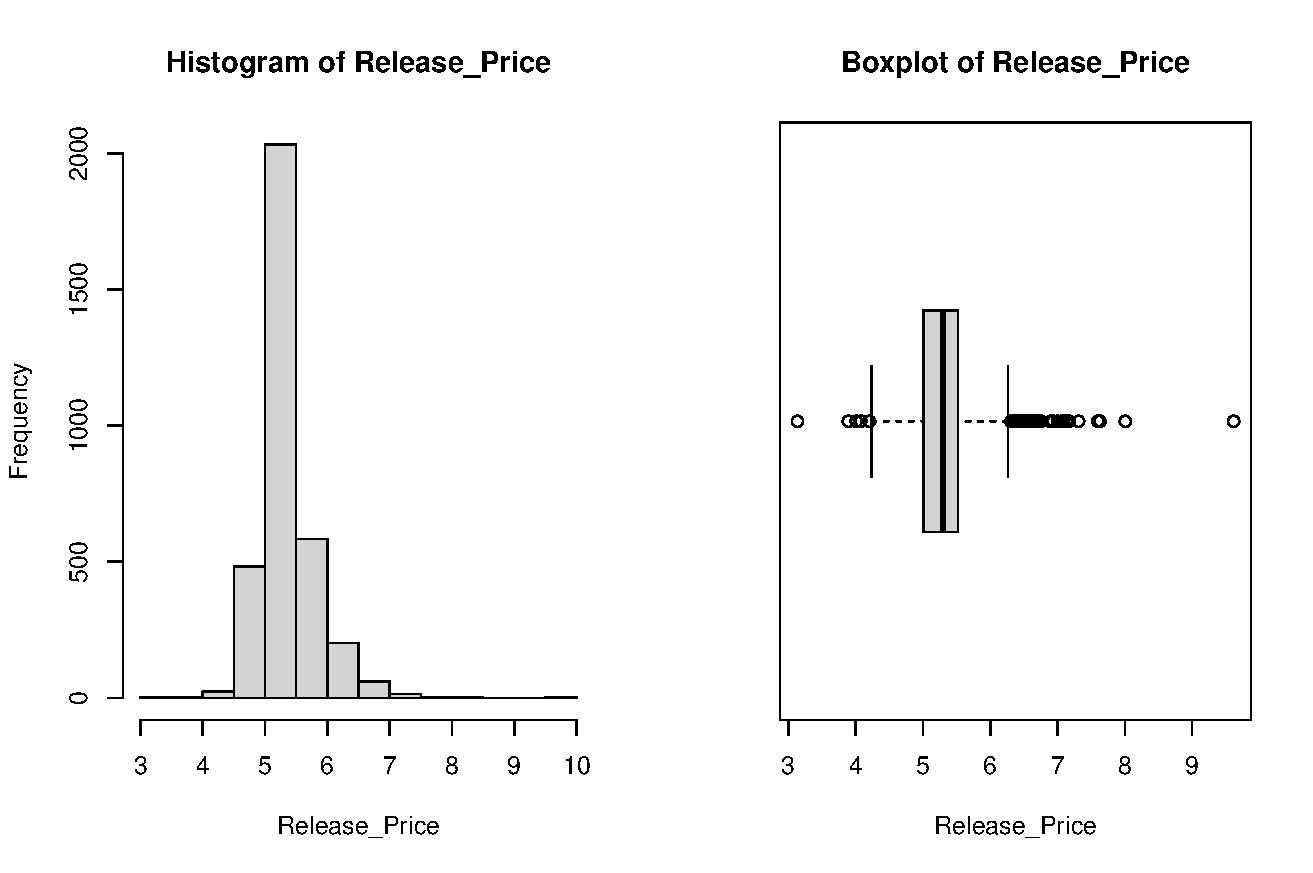
\includegraphics[keepaspectratio, width=1\textwidth, height=1\textheight]{Visualization/Rplot_18.pdf}\\
    \end{tabular}
\end{adjustbox}
\end{center}
\begin{center}
\begin{adjustbox}{width=\textwidth}
    \begin{tabular}{cc}
        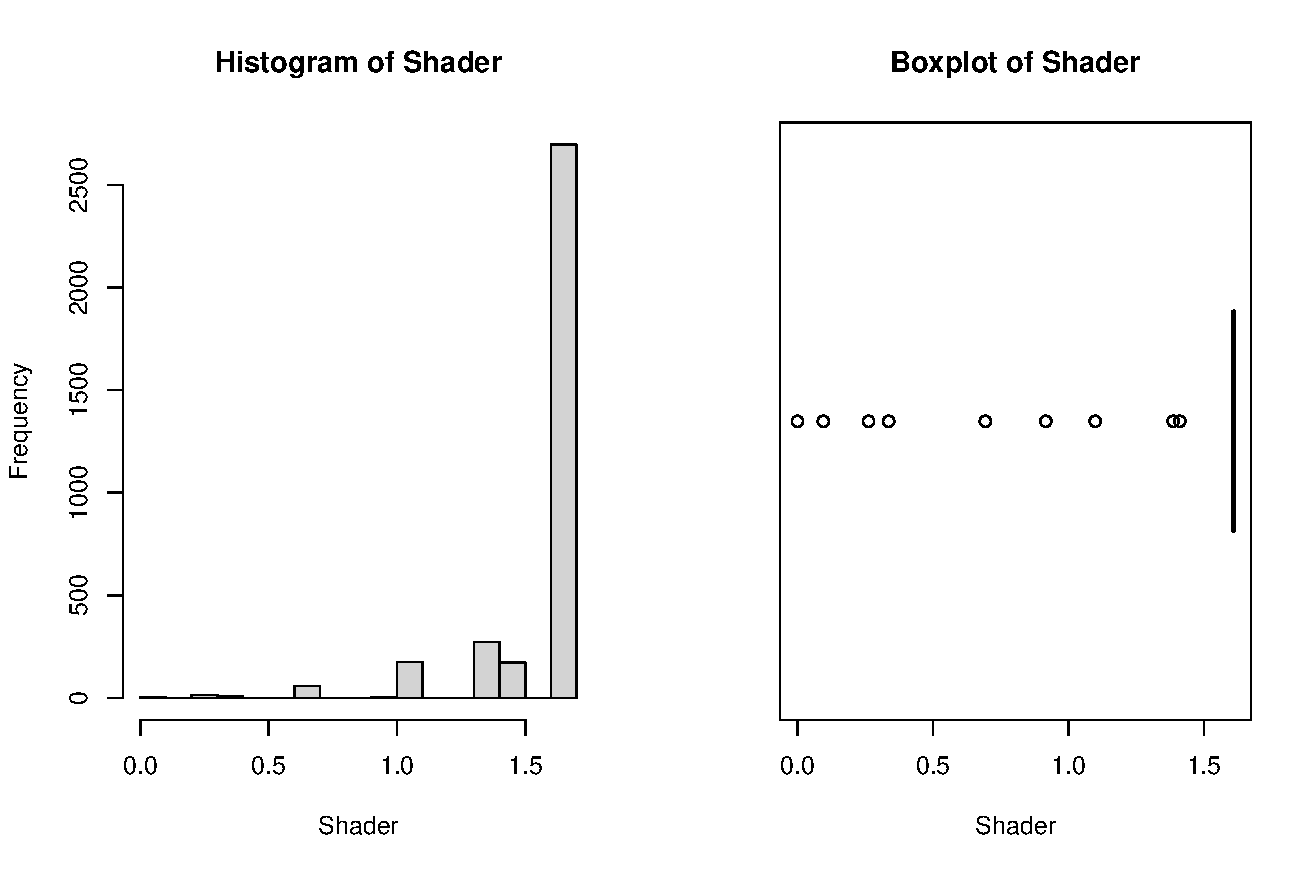
\includegraphics[keepaspectratio, width=1\textwidth, height=1\textheight]{Visualization/Rplot_19.pdf}
        &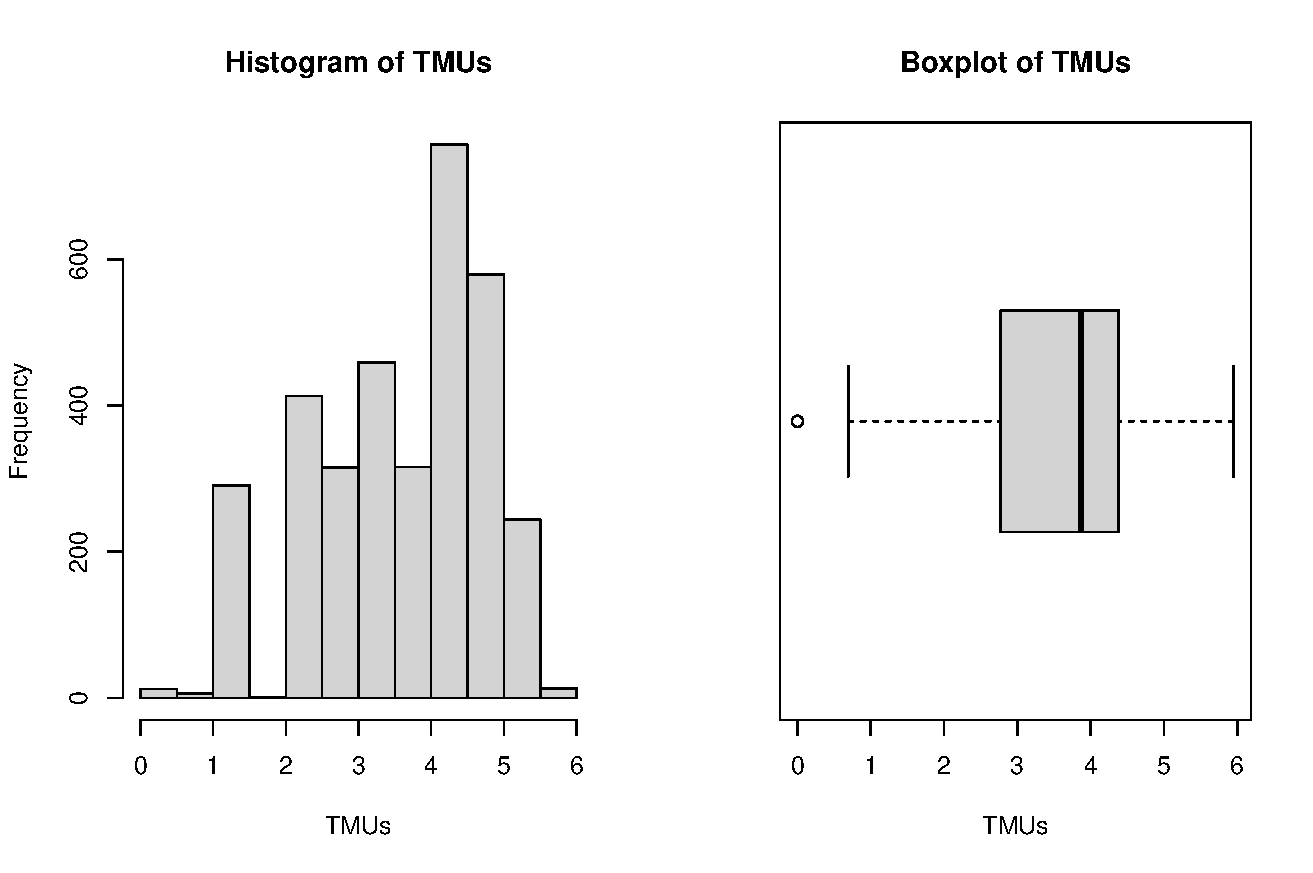
\includegraphics[keepaspectratio, width=1\textwidth, height=1\textheight]{Visualization/Rplot_20.pdf}\\
    \end{tabular}
\end{adjustbox}
\end{center}
Finally, not only Release\textunderscore Price but also most of other attributes are now normally distributed. Notice that the occurrences of $log(Release\textunderscore Price)\ge 8$ and $log(Release\textunderscore Price)\le 3.5$ is rare, so it should be eliminated in the next analysis. Now, we use Correlation plot to give the overview of the relation between each pair of variable after log\textunderscore transformation:\\
\begin{figure}[h!]
\begin{center}
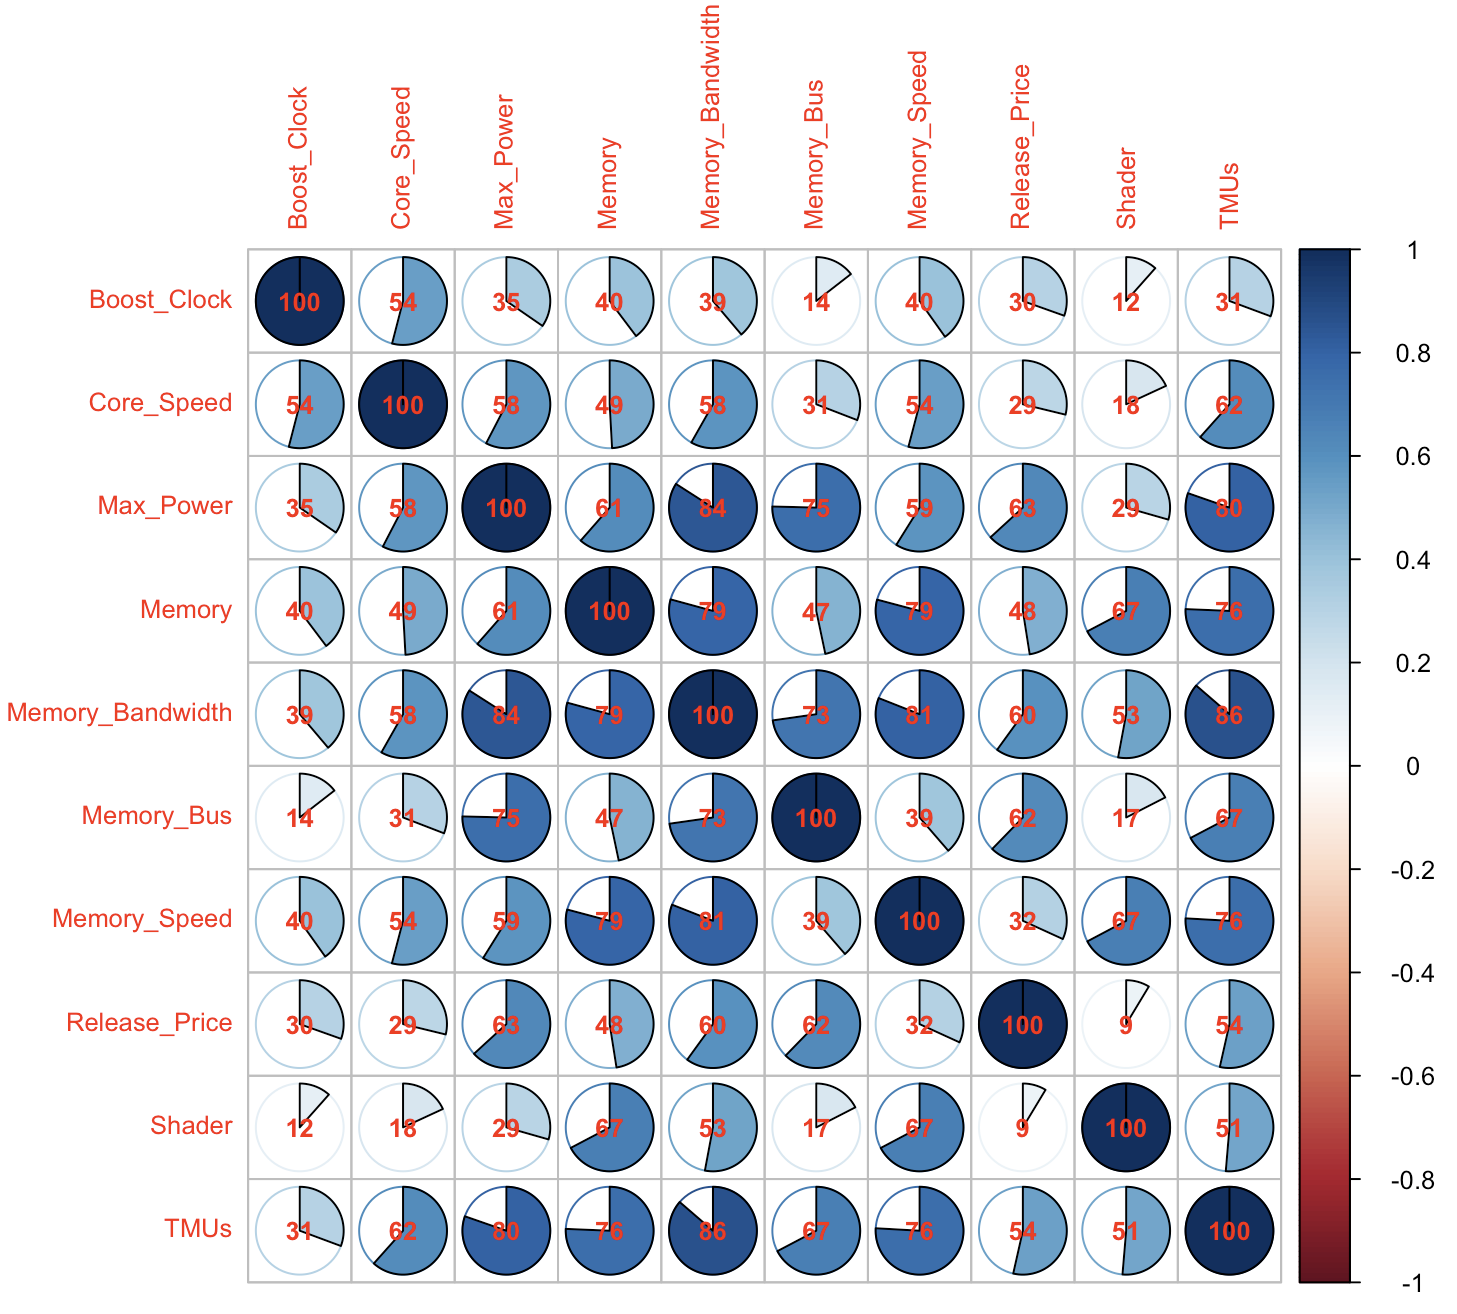
\includegraphics[width=14cm]{images/2.png}
\end{center}
\caption{Correlation Plot}
\end{figure}
\pagebreak
\begin{enumerate}
    \item \verb|Boost_Clock:|Strong positive correlation with Core\textunderscore Speed, which is expected as both involve operational speeds of the GPU. With attributes like Shader and TMUs, indicating that the boost clock speed is not significantly influenced by the number of shaders or texture mapping units.

    \item \verb|Core_Speed:| Strongly correlated with Boost\textunderscore Clock due to their related nature in defining GPU speeds. Shows weak correlation with Shader and TMUs, similar to Boost\textunderscore Clock.

     \item \verb|Max_Power:|Shows a strong positive correlation with Memory, suggesting that GPUs with higher power consumption tend to have more memory. Weak negative correlation with Memory\textunderscore Bus, indicating that higher power consumption does not necessarily mean a wider memory bus.

     \item \verb|Memory:| Strong positive correlations with Memory\textunderscore Bandwidth and Memory\textunderscore Speed, as more memory capacity typically supports higher bandwidth and speed. Relatively weak correlation with Shader, suggesting that the amount of memory is not directly related to the number of shaders.

     \item \verb|Memory_Bandwidth:|Highly correlated with Memory and Memory\textunderscore Speed, which is logical since higher bandwidth is often accompanied by higher memory speeds. Weak correlation with Shader and TMUs, showing that memory bandwidth is not closely related to these attributes.

      \item \verb|Memory_Bus:| Shows a strong correlation with Memory\textunderscore Speed, indicating that wider buses are often associated with faster memory speeds. Weak correlation with Max\textunderscore Power, suggesting that the width of the memory bus does not increase with power consumption.

      \item \verb|Memory_Speed:| Strongly correlated with Memory\textunderscore Bandwidth and Memory\textunderscore Bus, as faster memory speeds require higher bandwidth and potentially wider buses. Weak correlation with Shader and TMUs, indicating that memory speed is largely independent of these attributes.

      \item \verb|Release_Price:|Shows some correlation with Memory and Memory\textunderscore Bandwidth, suggesting that GPUs with more memory and higher bandwidth tend to be priced higher. Weak correlation with Shader, indicating that the number of shaders does not have a strong impact on the release price.

      \item \verb|Shader:| Shows some correlation with TMUs, as both are related to the rendering capabilities of GPUs. Very weak correlations with most other attributes like Boost\textunderscore Clock, Core\textunderscore Speed, and Memory, indicating that the number of shaders is quite independent of these features.

      \item \verb|TMUs:|Correlates with Shader, which is expected as both are involved in texture and rendering processes. Weak correlations with attributes like Boost\textunderscore Clock and Core\textunderscore Speed, showing that TMUs are not significantly influenced by the operational speeds of the GPU.
\end{enumerate}.
\pagebreak
\section{Inferential statistic}
\textbf{According to our team's discussion}, the main analysis attribute of this report is \textbf{Release\textunderscore Price} of the GPU and the effect of other attributes on this dependent variable. The reason why we choose this attribute is that price forecasting has played an increasingly important role in the ability of a company to remain competitive in the real world. Back to the project, we would try to utilize some Regression models to predict its Release\textunderscore Price via other configurations (or determinants).
\subsection{Data preparation}
First, again we load the clean dataset and log-transform it:
\begin{mdframed}[leftline=false,rightline=false,backgroundcolor=lightblue!10,nobreak=false]
    \begin{minted}[linenos,breaklines,breaksymbolleft=,obeytabs=true,tabsize=2]{R}
#inferential statistics
df <- read.csv("gpu_clean.csv")
df['Max_Power'] <- log(df['Max_Power'])
df['Boost_Clock'] <- log(df['Boost_Clock'])
df['Core_Speed'] <- log(df['Core_Speed'])
df['Memory'] <- log(df['Memory'])
df['Memory_Bandwidth'] <- log(df['Memory_Bandwidth'])
df['Memory_Bus'] <- log(df['Memory_Bus'])
df['Memory_Speed'] <- log(df['Memory_Speed'])
df['Release_Price'] <- log(df['Release_Price'])
df['Shader'] <- log(df['Shader'])
df['TMUs'] <- log(df['TMUs'])
    \end{minted}
\end{mdframed}
According to 3.2 and our statement previously, the occurrences of $log(Release\textunderscore Price)\ge 8$ and $log(Release\textunderscore Price)\le 3.5$ is rare is rare, so we will eliminate it from the dataset:
\begin{mdframed}[leftline=false,rightline=false,backgroundcolor=lightblue!10,nobreak=false]
    \begin{minted}[linenos,breaklines,breaksymbolleft=,obeytabs=true,tabsize=2]{R}
df <- df[df$Release_Price < 8,]
df <- df[df$Release_Price > 3.5,]
    \end{minted}
\end{mdframed}
Because we would make use of Regression models to capture the relationships, a Test Set and a Training Set must be present to perform cross-validation to test the fitness of the model. In machine learning, splitting the data into distinct sets helps prevent overfitting, which occurs when a model memorizes the training data too well and fails to generalize to new, unseen data. So that, we split the data into training and testing sets by 80\% and 20\% amount of data.
\begin{mdframed}[leftline=false,rightline=false,backgroundcolor=lightblue!10,nobreak=false]
    \begin{minted}[linenos,breaklines,breaksymbolleft=,obeytabs=true,tabsize=2]{R}
#predict: 
set.seed(50)
# use 80% of dataset as training and 20% as testing
sample <- sample(c(T, F), nrow(df), replace=T, prob=c(0.8,0.2))
    \end{minted}
\end{mdframed}
\subsection{Hypothesis Testing}
\subsubsection{One-way ANOVA}
In this section, we want to know whether or not a significant difference in the average Release\textunderscore Price among manufacturers. Then we are going to use function selection to filter the data based on the Release\textunderscore Price of each manufacturer in df:
\begin{mdframed}[leftline=false,rightline=false,backgroundcolor=lightblue!10,nobreak=false]
    \begin{minted}[linenos,breaklines,breaksymbolleft=,obeytabs=true,tabsize=2]{R}
aovRelease_Price <- select(df, Manufacturer, Release_Price)
    \end{minted}
\end{mdframed}
\textbf{ANOVA Test}\\
In order to determine if there is any significant difference in Release\textunderscore Price among these manufacturers, we enumerate the null hypothesis $H_{0}$ and alternative hypothesis $H_{1}$.
\begin{itemize}
    \item $H_{0}$: $u1 = u2 =...= u_{i} = 0$: There is a similarity in average Release\textunderscore Price among 4 manufacturers: Nvidia, AMD, Intel and ATI.
    \item $H_{1}$: $u_{i} \neq 0$ for at least one of the manufacturer have a significant different in Release\textunderscore Price compared to others.
\end{itemize}
\lstinputlisting[language={},numbers=none,caption={ANOVA}]{txt/7.txt}
We can see that as the \textbf{p-value $<$ 0.05}, we can reject the null hypothesis $H_{0}$ and accept the alternative hypothesis $H_{1}$.\\
To compute \textbf{one-way ANOVA test}, the data in df must be a fixed-impact model meet the follow requirements:
\begin{itemize}
    \item All data are independent and collected randomly, since the data is collected from 4 different manufacturers, so this condition is \textbf{satisfied}.
    \item The population from those samples should be normally distributed.
    \item Homogeneity of variance: the variance among the groups should be approximately equal.
\end{itemize}
Check \textbf{condition 2}, we will use Q-Q plot to see if the data is normally distributed.

\begin{figure}[h!]
\begin{center}
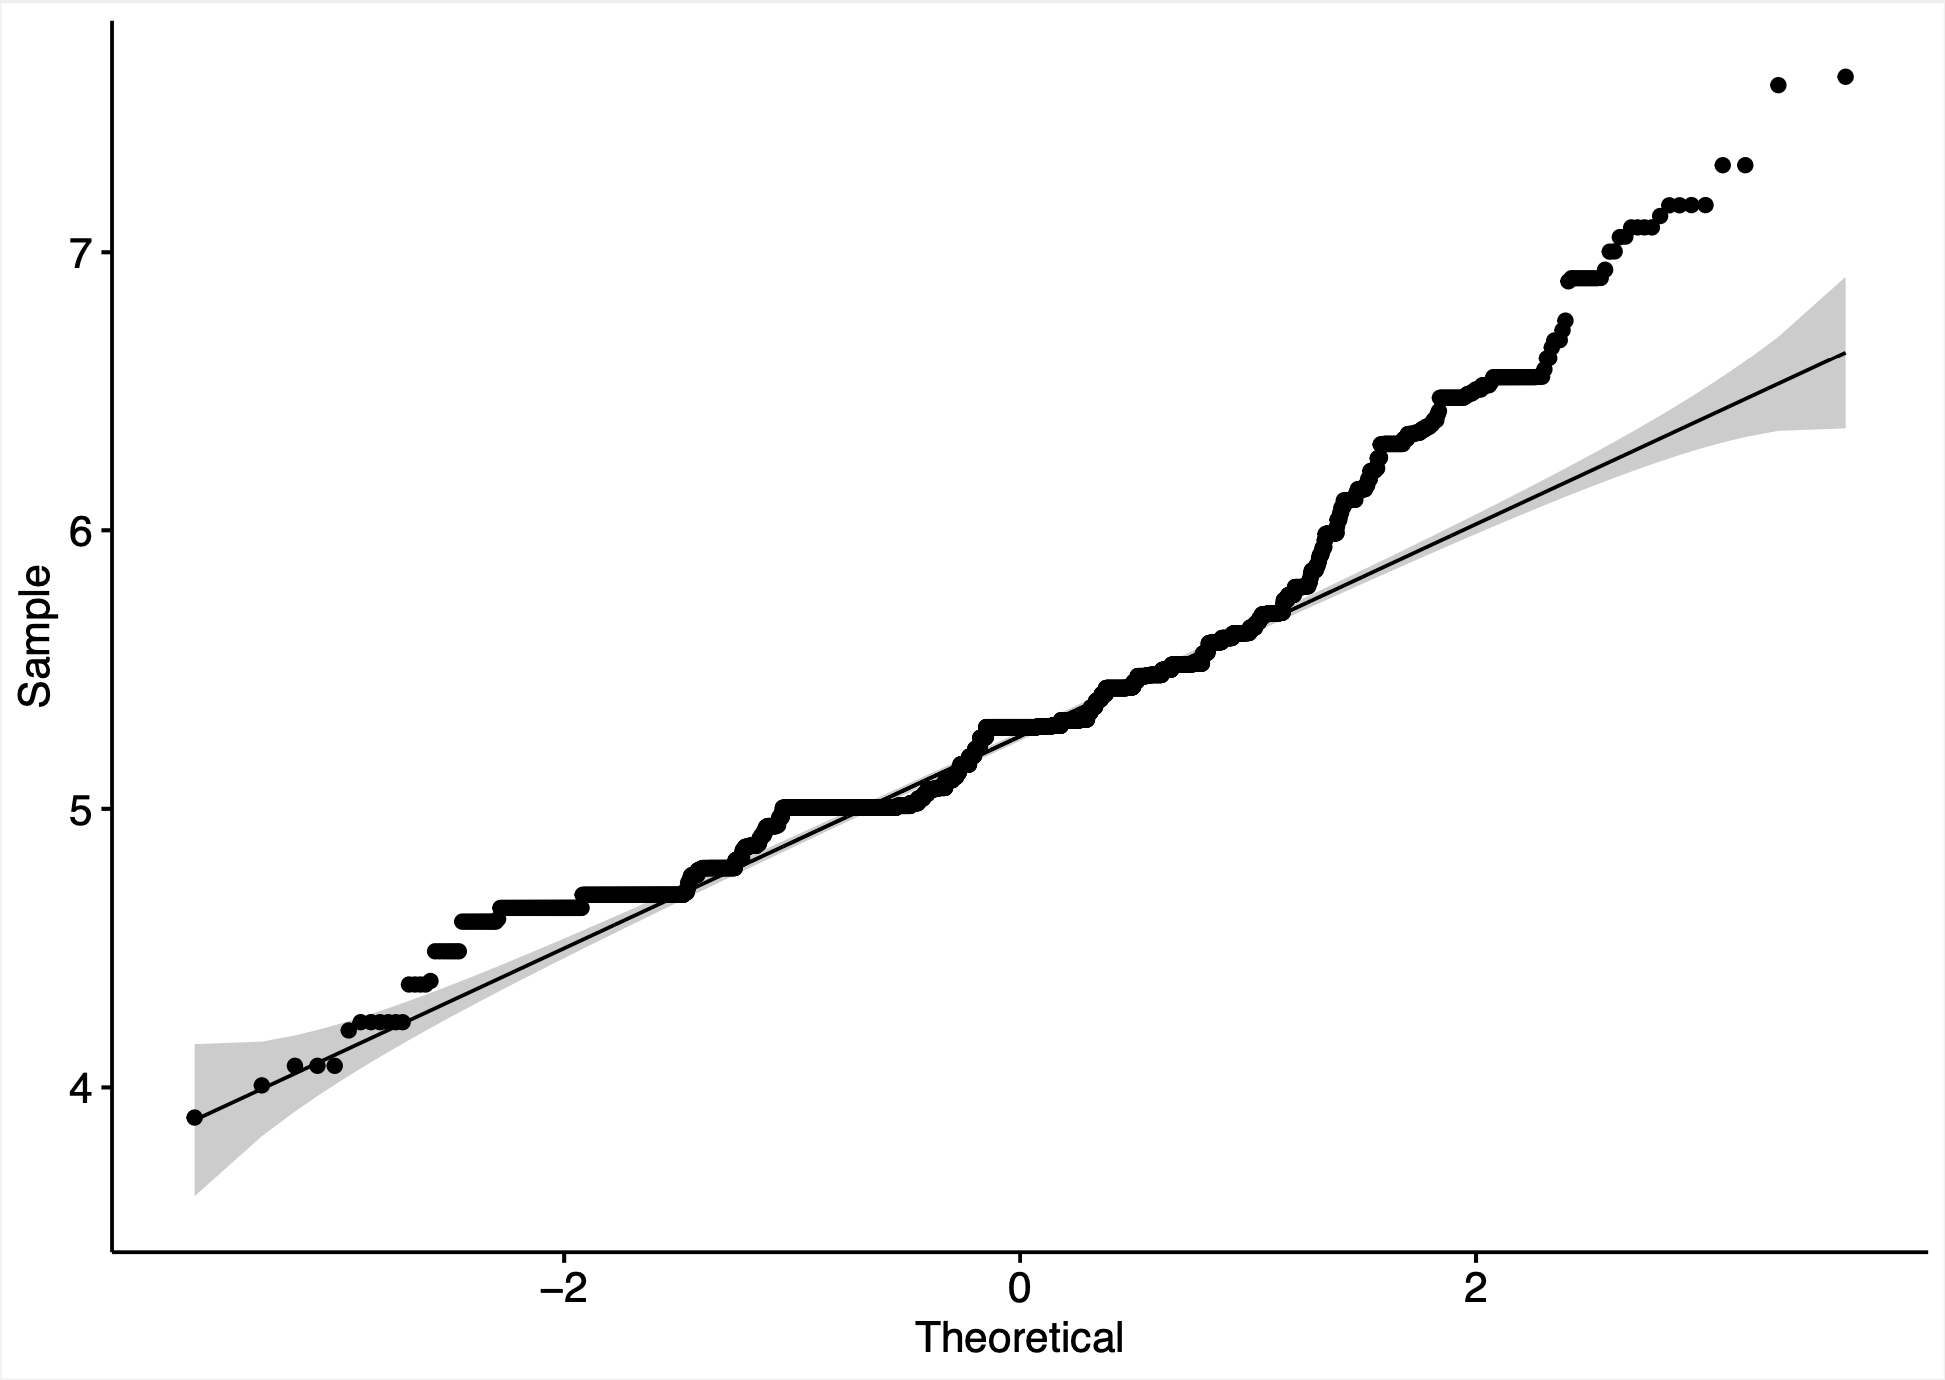
\includegraphics[width=11cm]{images/qqplot.png}
\end{center}
\caption{Q-Q plot for ANOVA}
\end{figure}
\\
\\
According to the plot provided, it can be seen that \textbf{Release\textunderscore Price} is not normally distributed. However, this assumption can be rejected since the sample size is large and the \textbf{Central Limit Theorem} ensures that the distribution of disturbance term will approximate normality. Also, \textbf{the one-way ANOVA} is considered a robust test against the normality assumption. This means that it tolerates violations to its normality assumption rather well. We can conclude that the second condition is \textbf{not necessarily satisfied}.\\
\\
Check \textbf{condition 3}, we will use \textbf{Levene-test} to evaluate if the variances of two populations are equal. Levene’s test is an inferential statistic used to evaluate the equality of variances for a variable determined by two or more groups. The statistical hypotheses are:
\begin{itemize}
    \item Null hypothesis $H_{0}$: All populations are equal.
    \item Alternative hypothesis $H_{1}$: At least two of them are different.
\end{itemize}
\lstinputlisting[language={},numbers=none,caption={Levene-test}]{txt/6.txt}
From the output above, we can see that the p-value ($<$ 2.2e-16) is much smaller compares to the alpha level 0.05. Now we reject the null hypothesis $H_{0}$ that all populations are equal, which also means there is a difference among manufacturers.\\
\\
\textbf{Welch's test}\\
\\
Since the variance test fail as its p-value is less than 0.05 and the qq-plot has a lot of point that deviate from the line, we will use Welch's test to check if the assumption is correct or not.
\begin{mdframed}[leftline=false,rightline=false,backgroundcolor=lightblue!10,nobreak=false]
    \begin{minted}[linenos,breaklines,breaksymbolleft=,obeytabs=true,tabsize=2]{R}
oneway.test(Release_Price ~ Manufacturer, data = aovRelease_Price)
    \end{minted}
\end{mdframed}
\lstinputlisting[language={},numbers=none,caption={Levene-test}]{txt/8.txt}
According to Welch's test result, we can officially claim that \textbf{there is a difference in average Release\textunderscore Price among manufacturers.}

\subsection{Multiple Linear Regression}
In this section, we will conduct an investigation on the relationship between Release\textunderscore Price with other features.
\subsubsection{Fitting the multi-linear model}
\begin{mdframed}[leftline=false,rightline=false,backgroundcolor=lightblue!10,nobreak=false]
    \begin{minted}[linenos,breaklines,breaksymbolleft=,obeytabs=true,tabsize=2]{R}
#MLR
data = df %>%
  select("Boost_Clock","Core_Speed","Max_Power","Memory","Memory_Bandwidth"
  ,"Memory_Bus","Memory_Speed","Release_Price","Shader","TMUs")
train <- data[sample, ]
test <- data[!sample, ]
mdl_price_vs_all = lm(Release_Price~., data=train)
summary(mdl_price_vs_all)
    \end{minted}
\end{mdframed}
The \textbf{summary()} gives an overview over some statistics in our model.
\lstinputlisting[language={},numbers=none,caption={Summary of linear model}]{txt/9.txt}
It can be observed that no variable have \textbf{p-value $\ge$ 0.05}, which means all predictors that we have chosen is involved in the building process.
\subsubsection{Homoscedasticity checking}
Now we must check for Multi-Linear model assumption: 
\begin{enumerate}
    \item Residual Errors have a Mean Value of Zero.
    \item Residual Errors have Constant Variance.
    \item The errors are normally distributed.
\end{enumerate}
\textbf{Testing for Residual Errors have a Mean Value of Zero:} We can check the residuals by plotting their histograms and distributions.

\begin{figure}[h!]
\begin{center}
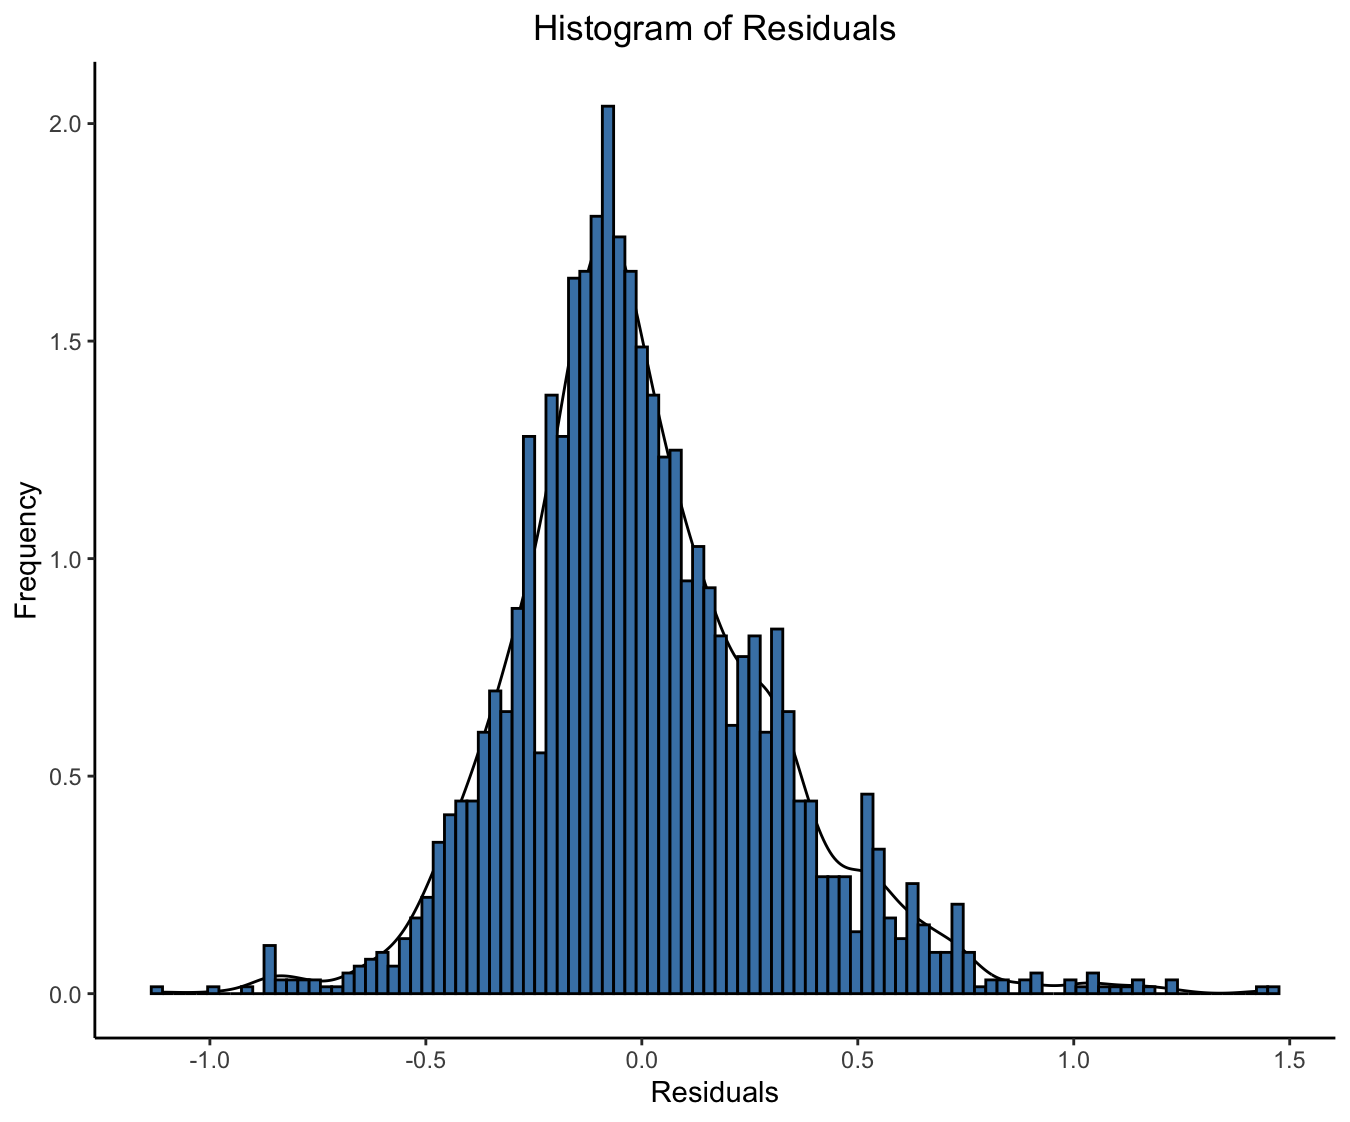
\includegraphics[width=7cm,length=8cm]{images/hist.png}
\end{center}
\caption{Histogram of residuals}
\end{figure}
\pagebreak
From the above figure, we can see a “fair” normal distribution because residuals distribute mainly around value 0. Based on these residuals, we can say that our model meets the assumption.\\
\\
\textbf{Testing for Residual Errors have Constant Variance:} We can check this assumption using the Scale-Location plot. In this plot we can see the fitted values vs the square root of the standardized residuals. Ideally, we would want to see the residual points equally spread around the red line, which would indicate constant variance.
\begin{mdframed}[leftline=false,rightline=false,backgroundcolor=lightblue!10,nobreak=false]
    \begin{minted}[linenos,breaklines,breaksymbolleft=,obeytabs=true,tabsize=2]{R}
plot(mdl_price_vs_all, which = 3)
\end{minted}
\end{mdframed}
\begin{figure}[h!]
\begin{center}
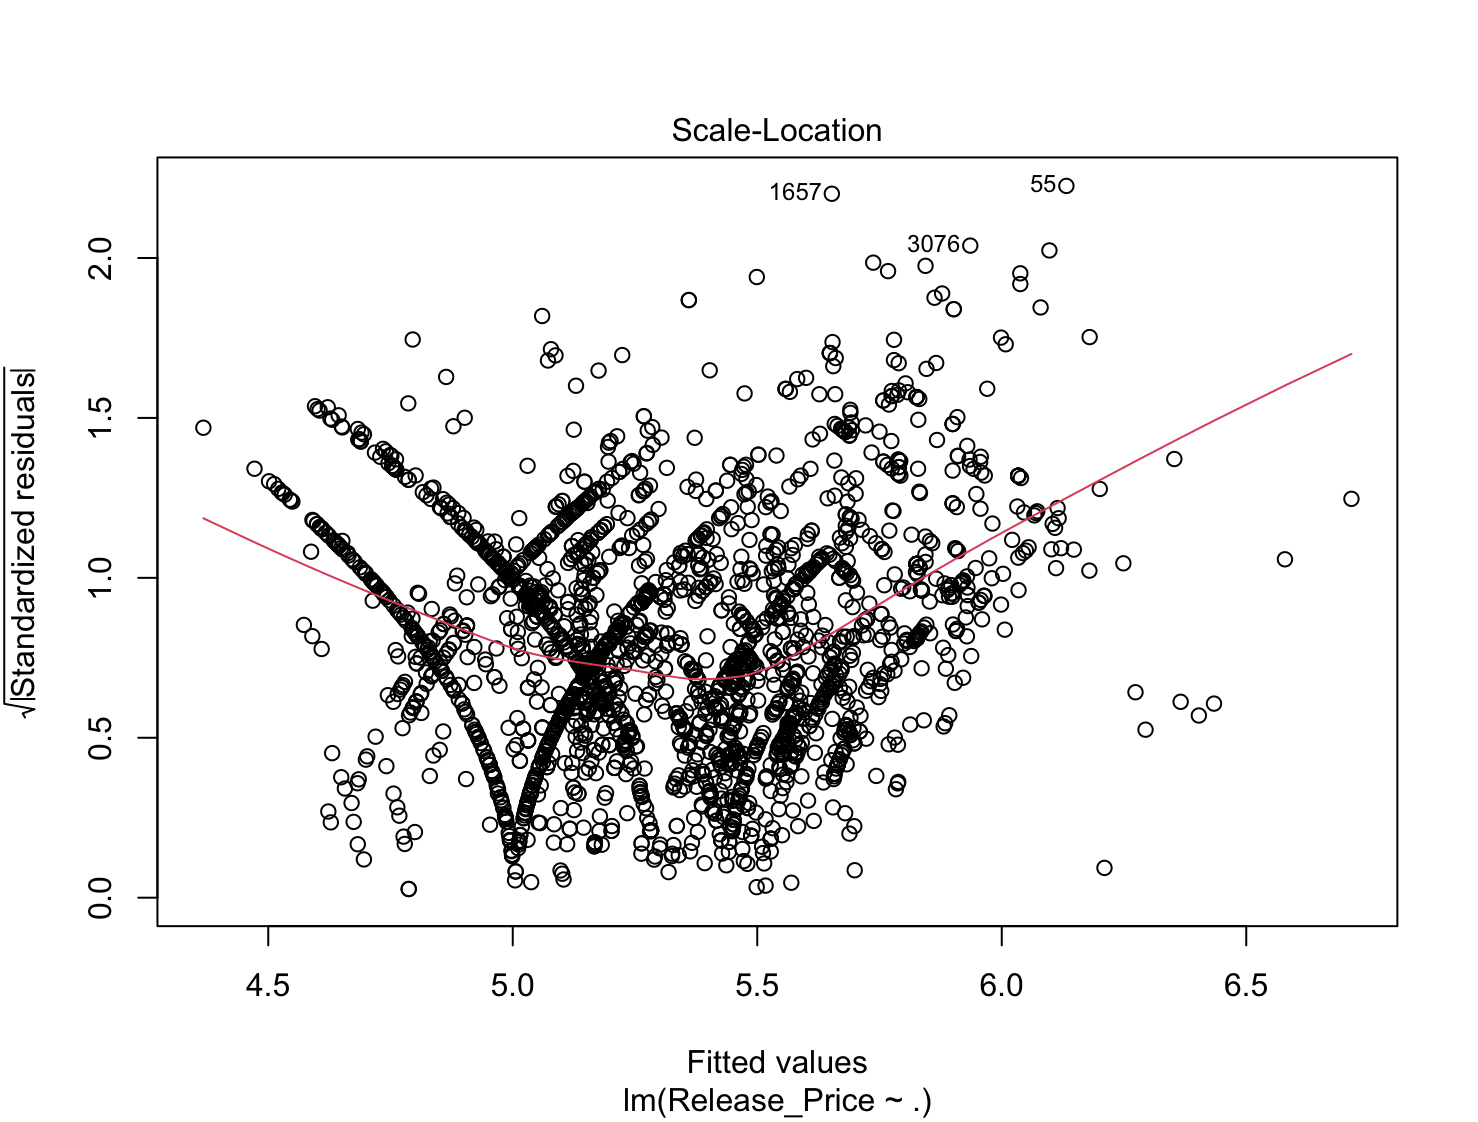
\includegraphics[width=8cm,height=5cm]{images/scale_l.png}
\end{center}
\caption{Scale-Location plot}
\end{figure}
In the above plot, the residuals scatter is not following any formal distribution and it do spread around the red line. So the assumption is approved.\\
\\
\textbf{Testing for normality of the the errors:} To check this, we have to use Q-Q plot for normality consideration. The output we expect that the residuals will mostly scatter close to the straight line to get normality hypothesis accepted.
\begin{mdframed}[leftline=false,rightline=false,backgroundcolor=lightblue!10,nobreak=false]
    \begin{minted}[linenos,breaklines,breaksymbolleft=,obeytabs=true,tabsize=2]{R}
plot(mdl_price_vs_all, which = 2)
\end{minted}
\end{mdframed}
\begin{figure}[h!]
\begin{center}
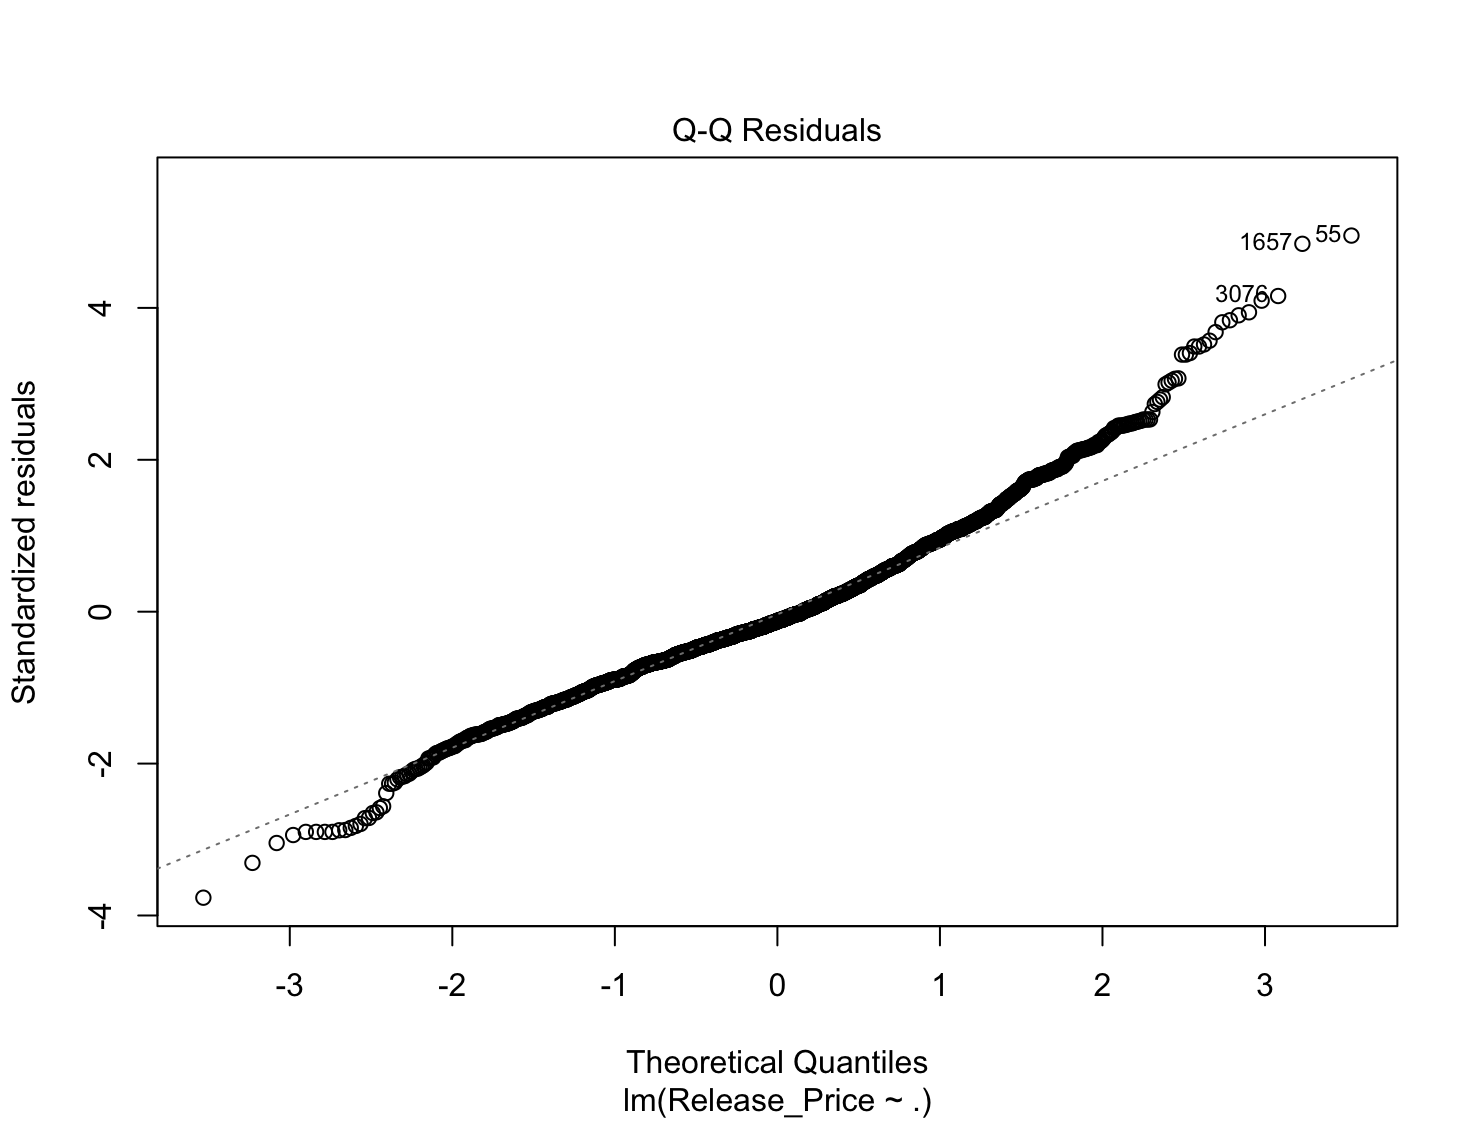
\includegraphics[width=8cm]{images/qq.png}
\end{center}
\caption{Q-Q plot}
\end{figure}
In the Q-Q plot, it can be seen that those points are lying near the line, while only a few points are not lying near the line. We can conclude that this model can be normally accurate.
\subsubsection{Linear equation}
\lstinputlisting[language={},numbers=none,caption={Coeff() function}]{txt/10.txt}
From listing 10, we can conclude that our linear equation will be(since we did log-transform at the beginning, so we should add exp and log to the equation):
\begin{mdframed}[leftline=false,rightline=false,backgroundcolor=lightblue!10,nobreak=false,numbers=false]
    \begin{minted}[linenos,breaklines,breaksymbolleft=,obeytabs=true,tabsize=2]{R}
Release_Price=exp(4.40184988+0.42684428*log(Boost_Clock)-0.26377554*log(Core_Speed)
+0.09983657*log(Max_Power)+0.13631975*log(Memory)+0.16804059*log(Memomy_Bandwidth)
+0.09096643*log(Memory_Bus)-0.32001565*log(Memory_Speed)-0.60688925*log(Shader)
+0.05911582*log(TMUs))
\end{minted}
\end{mdframed}
\subsubsection{Model prediction}
We will do the scatter plotting for the predicted value of test set compared with real values of the dataset using plot() function for more clear vision of this trend.\\
\begin{figure}[h!]
\begin{center}
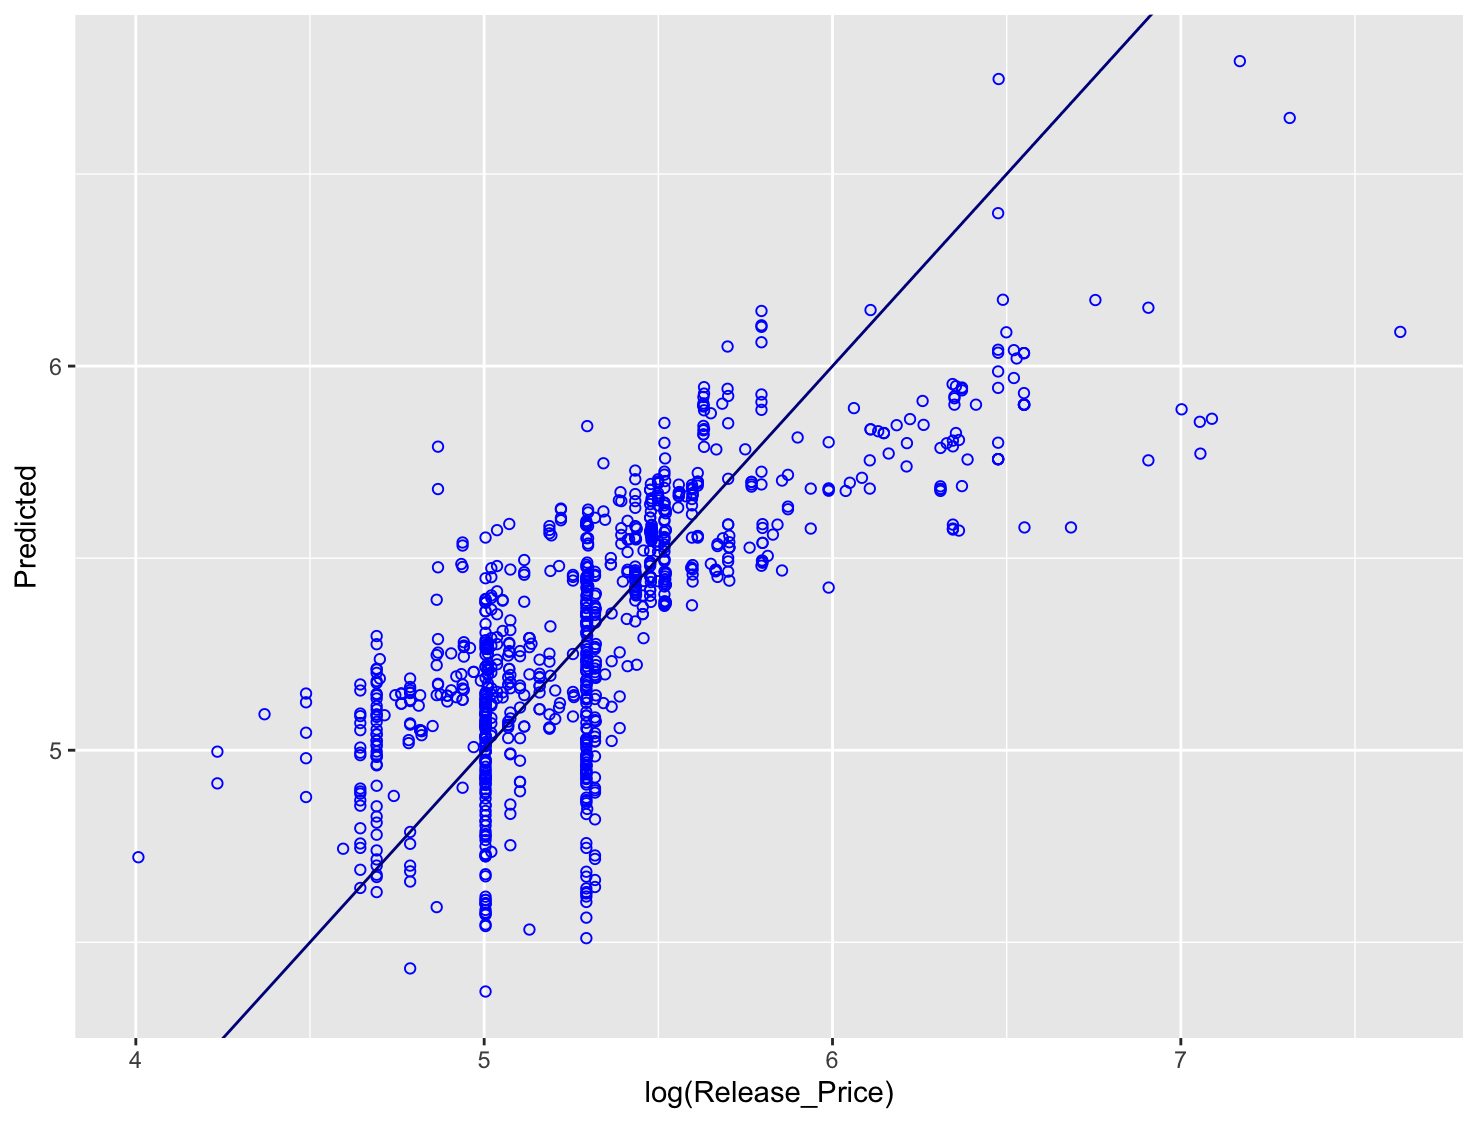
\includegraphics[width=10cm]{images/pre_log.png}
\end{center}
\caption{Prediction plot}
\end{figure}
\\
The plotted line in graph is (d) : y = x. The more concentration on this line the more correct the model does. To be more specific, we will show 10 values with their predicted : \\
\lstinputlisting[language={},numbers=none,caption={Comparison of testing and predicting value}]{txt/11.txt}
The top 10 above predicted values are not really close to the test\textunderscore set and the accuracy of the whole test set is only 56.73\%, which means this model is not \textbf{accurate}. 
\begin{mdframed}[leftline=false,rightline=false,backgroundcolor=lightblue!10,nobreak=false,numbers=false]
    \begin{minted}[linenos,breaklines,breaksymbolleft=,obeytabs=true,tabsize=2]{R}
> SSE <- sum((test$Release_Price - pred)^2)
> SST <- sum((test$Release_Price - mean(test$Release_Price))^2)
> cat("The accuracy of the model on test set: " , round((1 - SSE / SST )* 100 ,2) , "%" )
The accuracy of the model on test set:  56.73 %
\end{minted}
\end{mdframed}
\pagebreak
\section{Discussion and extension}
\subsection{Multiple Linear Regression}
\subsubsection{Advantages}
The biggest advantage of linear regression models is linearity: It makes the estimation procedure simple and, most importantly, these linear equations have an easy to understand interpretation on a modular level. The mathematical equation of Linear Regression is also fairly easy to understand and interpret.
\subsubsection{Disadvantages}
Multiple linear regression, like any statistical method, has its limitations and disadvantages. Here are some of them:

\begin{enumerate}
    \item \verb|Assumption of Linearity:| Multiple linear regression assumes that the relationship between the independent variables and the dependent variable is linear. If this assumption is violated, the model's predictions may be inaccurate.
    \item \verb|Assumption of Independence:| Multiple linear regression assumes that the independent variables are independent of each other. If there is multicollinearity (high correlation) among the independent variables, it can lead to unreliable estimates of the regression coefficients.
    \item \verb|Interpretability:| As the number of independent variables increases, it becomes more challenging to interpret the coefficients of the model. Understanding the individual impact of each independent variable on the dependent variable becomes less straightforward.
    \item \verb|Sensitive to Outliers:| Multiple linear regression can be sensitive to outliers, which are data points that deviate significantly from the rest of the data. Outliers can have a disproportionate influence on the estimated regression coefficients and may lead to misleading results.
    \item \verb|Assumption of Homoscedasticity:| Multiple linear regression assumes that the residuals (the differences between the observed and predicted values) have constant variance across all levels of the independent variables. Violation of this assumption, known as heteroscedasticity, can lead to biased standard errors and confidence intervals.
    \item \verb|Non-linearity of the Relationship:| While multiple linear regression assumes a linear relationship between the independent variables and the dependent variable, this may not always be the case in reality. In such situations, the model may not accurately capture the true relationship between the variables.
\end{enumerate}

Linear regression may not be the appropriate choice in certain situations, particularly when the assumptions of the model are violated or when the relationship between the variables is not linear. For instance, when dealing with data that exhibit a nonlinear relationship, such as exponential or polynomial patterns, linear regression may yield inaccurate predictions and unreliable parameter estimates. Because of that, we will try other models in the \textbf{extension} part.
\subsection{Extension}
\subsubsection{SVM model}
Support Vector Machine (SVM) is a supervised machine learning algorithm used for both classification and regression. In the project, we will try to build SVM model.
\lstinputlisting[language={},numbers=none,caption={Comparison of testing and predicting value}]{txt/12.txt}
\begin{mdframed}[leftline=false,rightline=false,backgroundcolor=lightblue!10,nobreak=false,numbers=false]
    \begin{minted}[linenos,breaklines,breaksymbolleft=,obeytabs=true,tabsize=2]{R}
> predictions_svm <- predict(svm_model, newdata = test)
> SSE_svm <- sum((predictions_svm - test$Release_Price)^2)
> SST_svm <- sum((test$Release_Price - mean(test$Release_Price))^2)
> r2_score <- 1 - SSE_svm / SST_svm
> print(paste("The accuracy of the model on test set: ",r2_score))
[1] "The accuracy of the model on test set:  0.83715919086462"
\end{minted}
\end{mdframed}
After modelling, when comparing test\textunderscore set and prediction, we can see that the prediction values have a small residual due to actual value. Even more, the accuracy is \textbf{84\%}, which means this model is more reliable than MLR.\\
Now we will check whether the residuals of the model is normally distributed or not using Q-Q plot.
\begin{figure}[h!]
\begin{center}
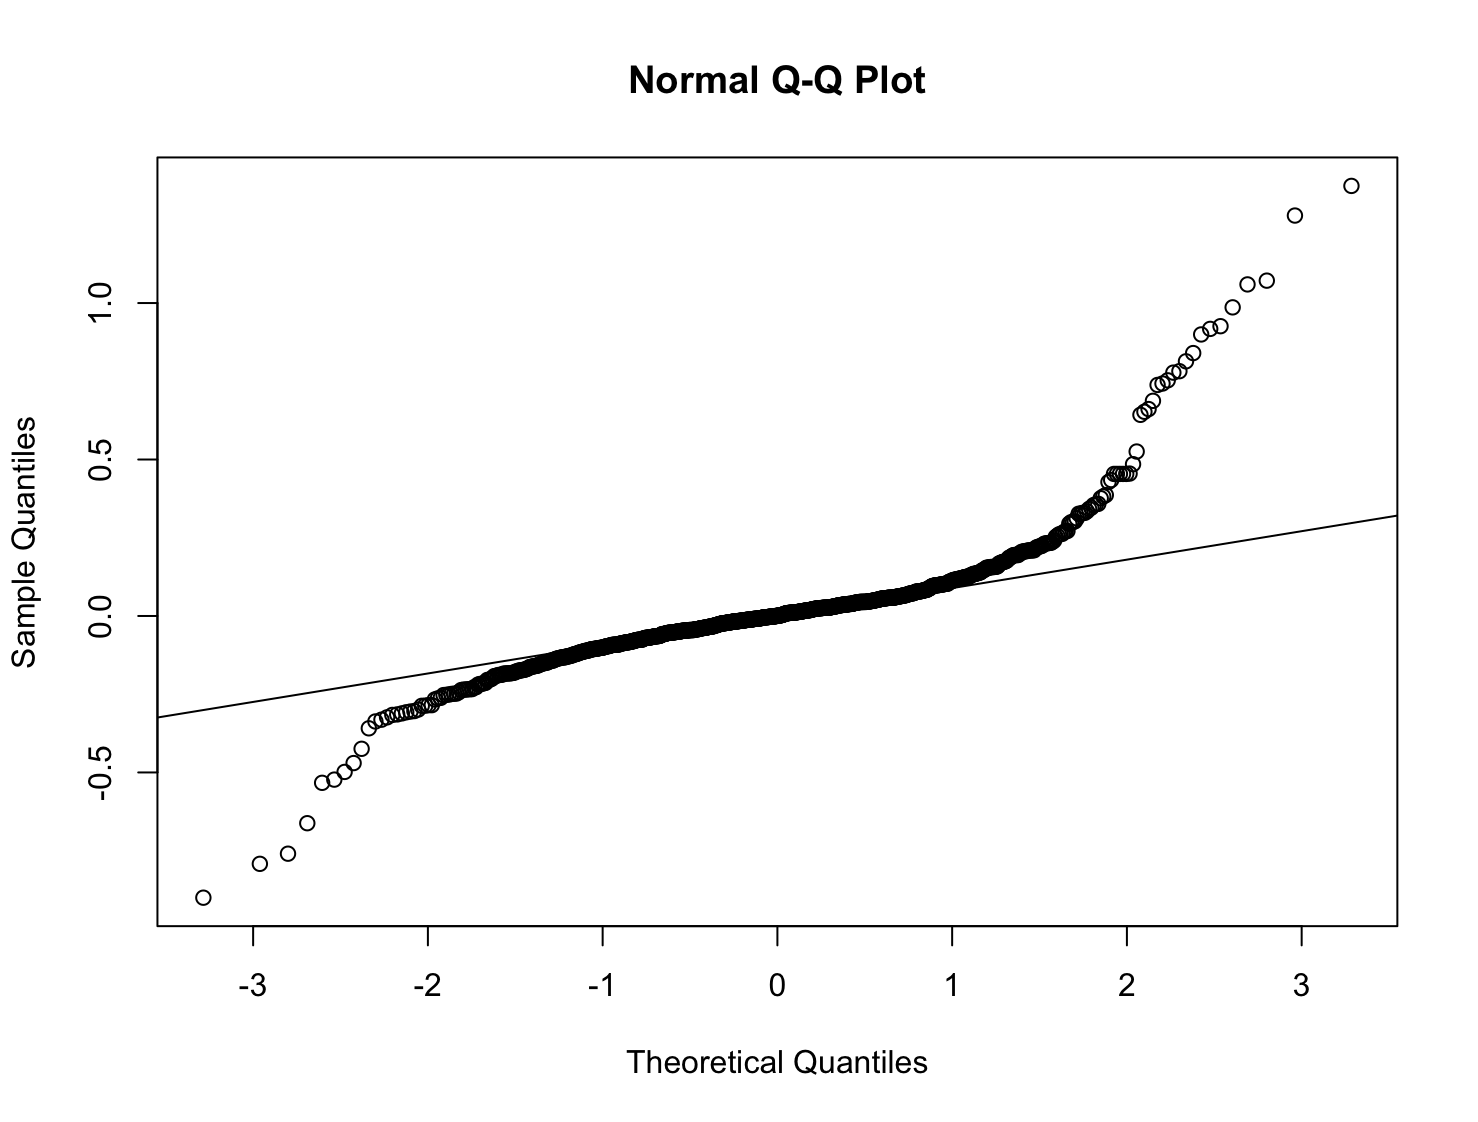
\includegraphics[width=10cm]{images/qqsvm.png}
\end{center}
\caption{SVM prediction plot}
\end{figure}
\\
Although all points are not fully lying near the line, most of them does. We conclude that this model is normally accurate.\\
We will do the scatter plotting for the predicted value of test set compared with real values of the test data set using plot() function:\\
\begin{figure}[h!]
\begin{center}
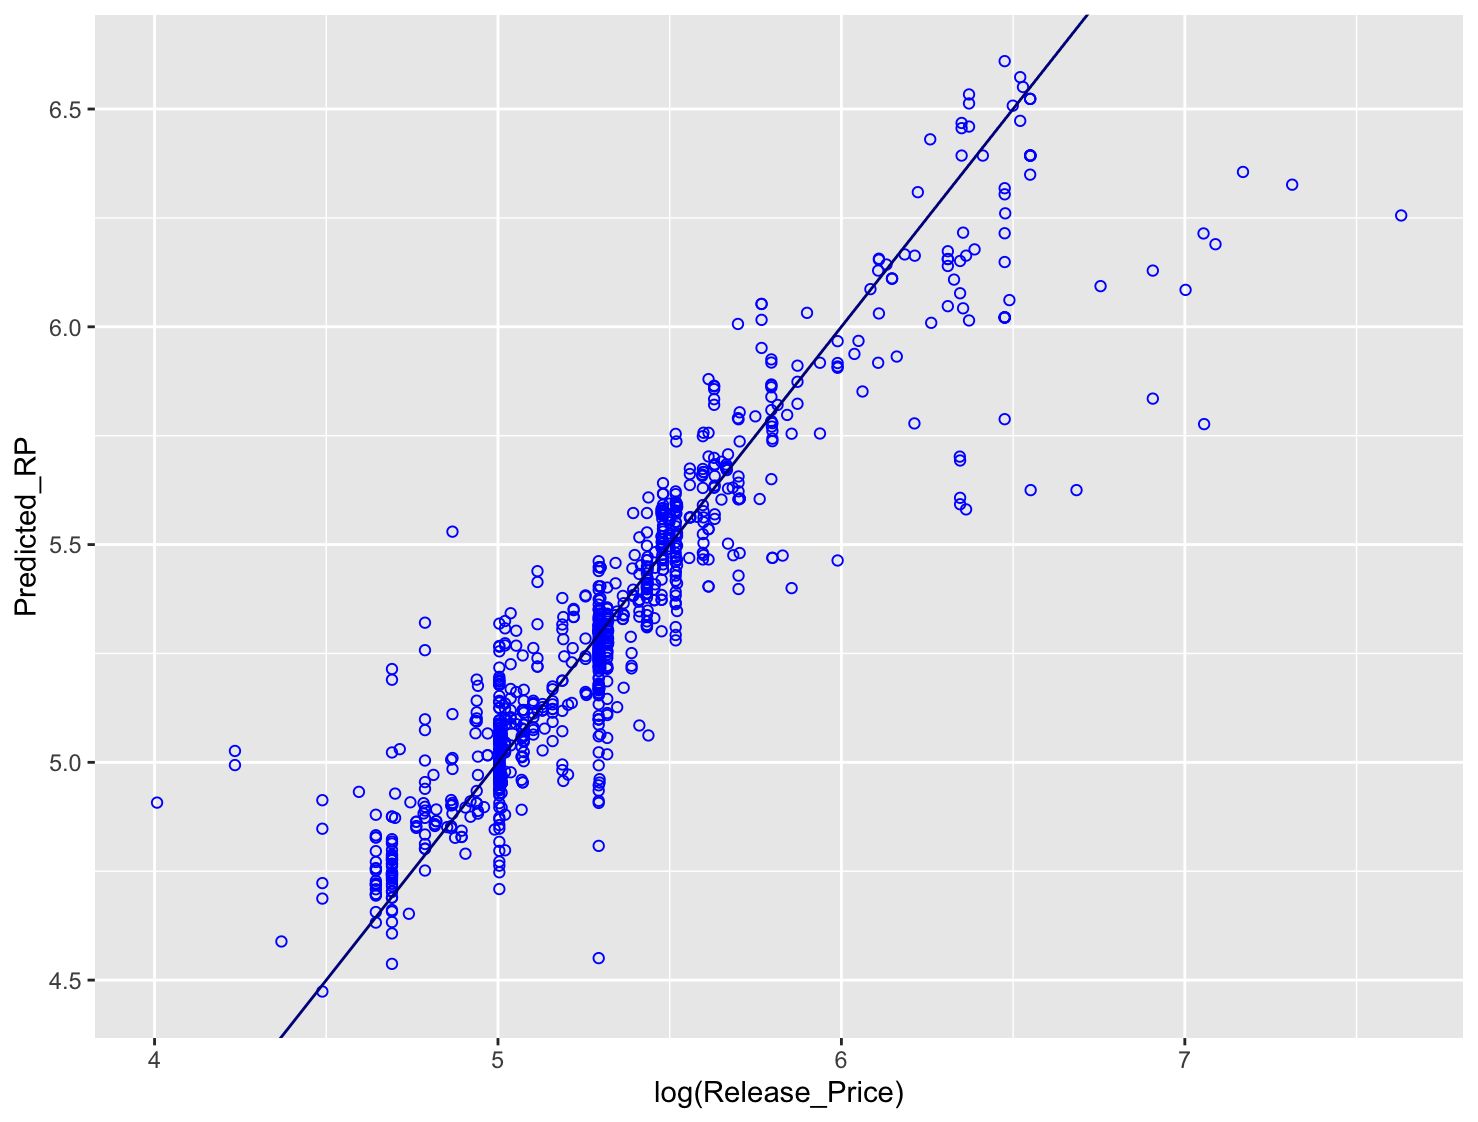
\includegraphics[width=10cm]{images/svm.png}
\end{center}
\caption{SVM prediction plot}
\end{figure}
\pagebreak
\\
As we can see, the closer the points to the line, the more accurate the prediction, and we clearly see, similarly to the previous model, there are more points close to the line than MLR, which is explained SVM is better than MLR.
\subsubsection{Random Forest Regression}
Random Forest Regression models are often used for predicting system performance metric. This algorithm can handle both continuous and categorical data. First, we will build the Random Forest regression model:
\begin{mdframed}[leftline=false,rightline=false,backgroundcolor=lightblue!10,nobreak=false,numbers=false]
    \begin{minted}[linenos,breaklines,breaksymbolleft=,obeytabs=true,tabsize=2]{R}
library("randomForest")
model.rfr <- randomForest(formula = Release_Price ~ ., data = train, ntree = 500)
print(model.rfr)
\end{minted}
\end{mdframed}
\lstinputlisting[language={},numbers=none,caption={Summary of Random Forest model}]{txt/14.txt}
In the output above, the “\% Var explained” (percentage of variance explained) is a measure of the amount of variation in the target variable that is explained by the random forest regression model. Specifically, it represents the percentage of the total variance in the target variable that is accounted for by the model, and a higher percentage of variance explained is considered better, as it indicates that the model is able to explain a larger proportion of the variation in the target variable.\\
A \% variance explained of \textbf{88.46\%} is generally considered to be a good result for a random forest regression model, as it suggests that the model is able to explain a significant amount of the variation in the target variable.\\
Now, we will check the accuracy of this model using \textbf{r2\textunderscore score}:
\begin{mdframed}[leftline=false,rightline=false,backgroundcolor=lightblue!10,nobreak=false,numbers=false]
    \begin{minted}[linenos,breaklines,breaksymbolleft=,obeytabs=true,tabsize=2]{R}
> comtab.rfr <- test['Release_Price']
> comtab.rfr['RP_predicted'] <- as.data.frame(predict(model.rfr, newdata = test), row.names = NULL)
> # Evaluate model performance
> SSE <- sum((comtab.rfr$Release_Price - comtab.rfr$RP_predicted)^2)
> SST <- sum((comtab.rfr$Release_Price - mean(comtab.rfr$Release_Price))^2)
> cat("The accuracy of the model on test set: " , round((1 - SSE / SST )* 100 ,2) , "%" )
The accuracy of the model on test set:  88.15 %
\end{minted}
\end{mdframed}
With the accuracy of 88.15\%, it is clear that this random forest regression model is better than SVM model and Multi-Linear Regression in overall. However, it is required to check whether this model's residual is normally distributed. Once again, we will use the Q-Q plot.
\begin{figure}[h!]
\begin{center}
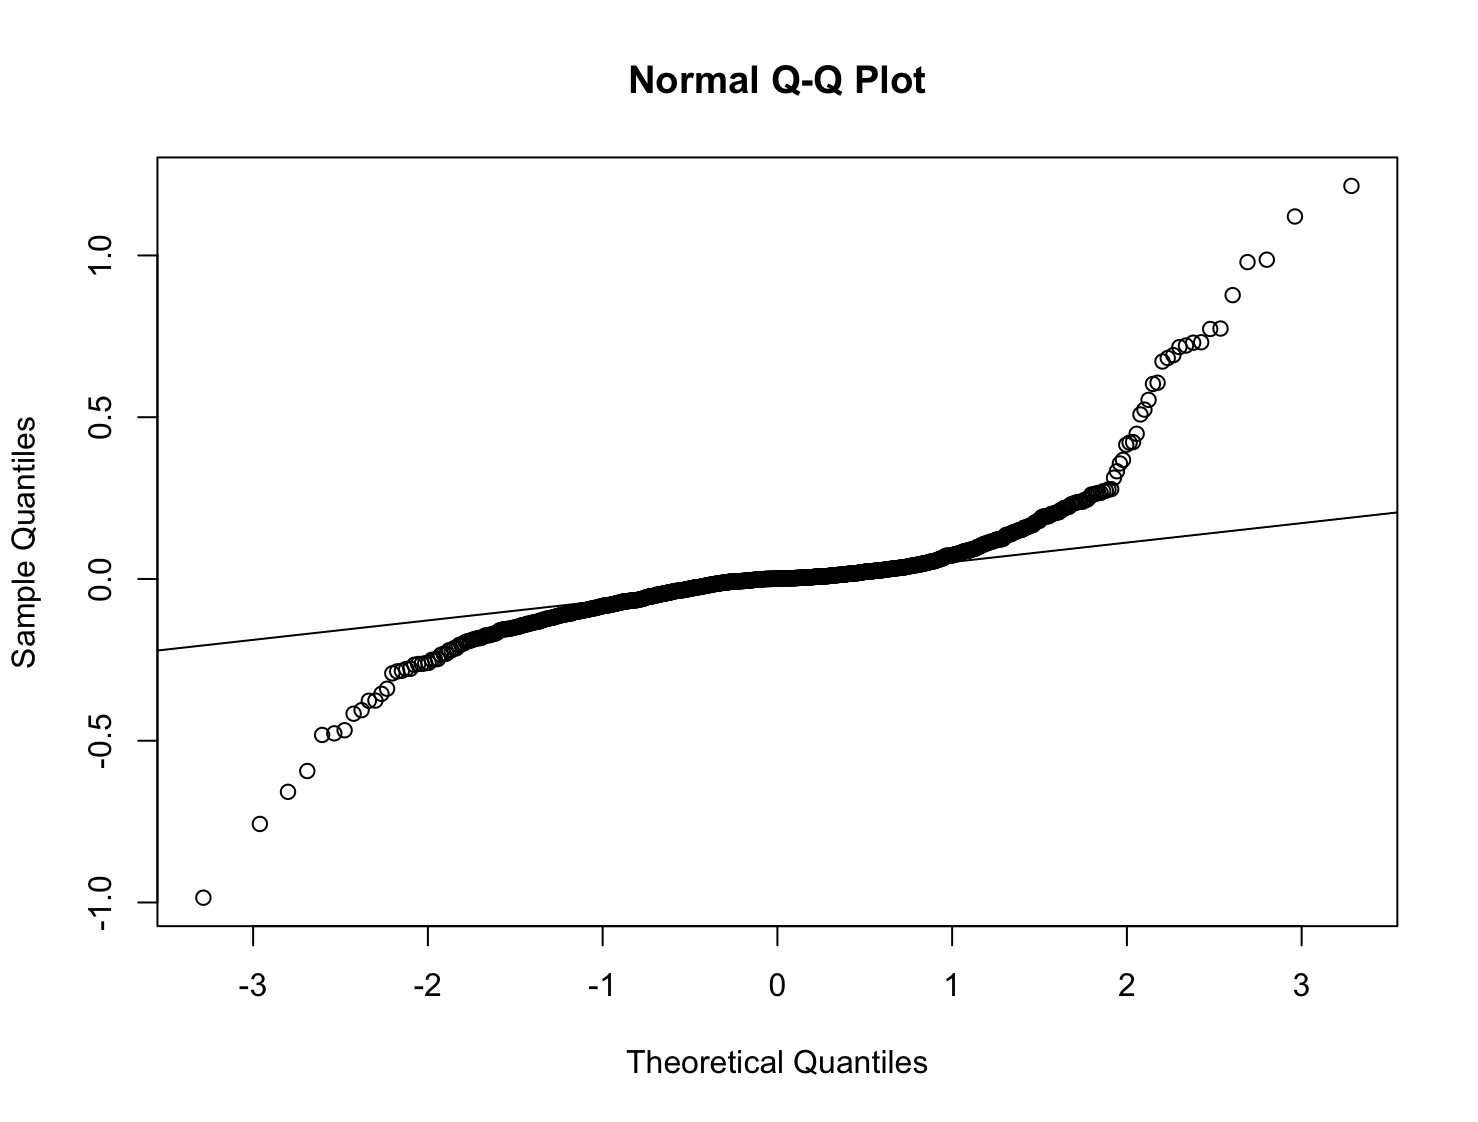
\includegraphics[width=10cm]{images/qqplot_rfr.png}
\end{center}
\caption{Q-Q plot of random forest regression}
\end{figure}
\\
\\
According to the above plot, we can conclude that this model is normally distributed while there are some outliers.\\
We will do the scatter plotting for the predicted value of test set compared with real values of
the test data set using plot() function:\\

\begin{figure}[h!]
\begin{center}
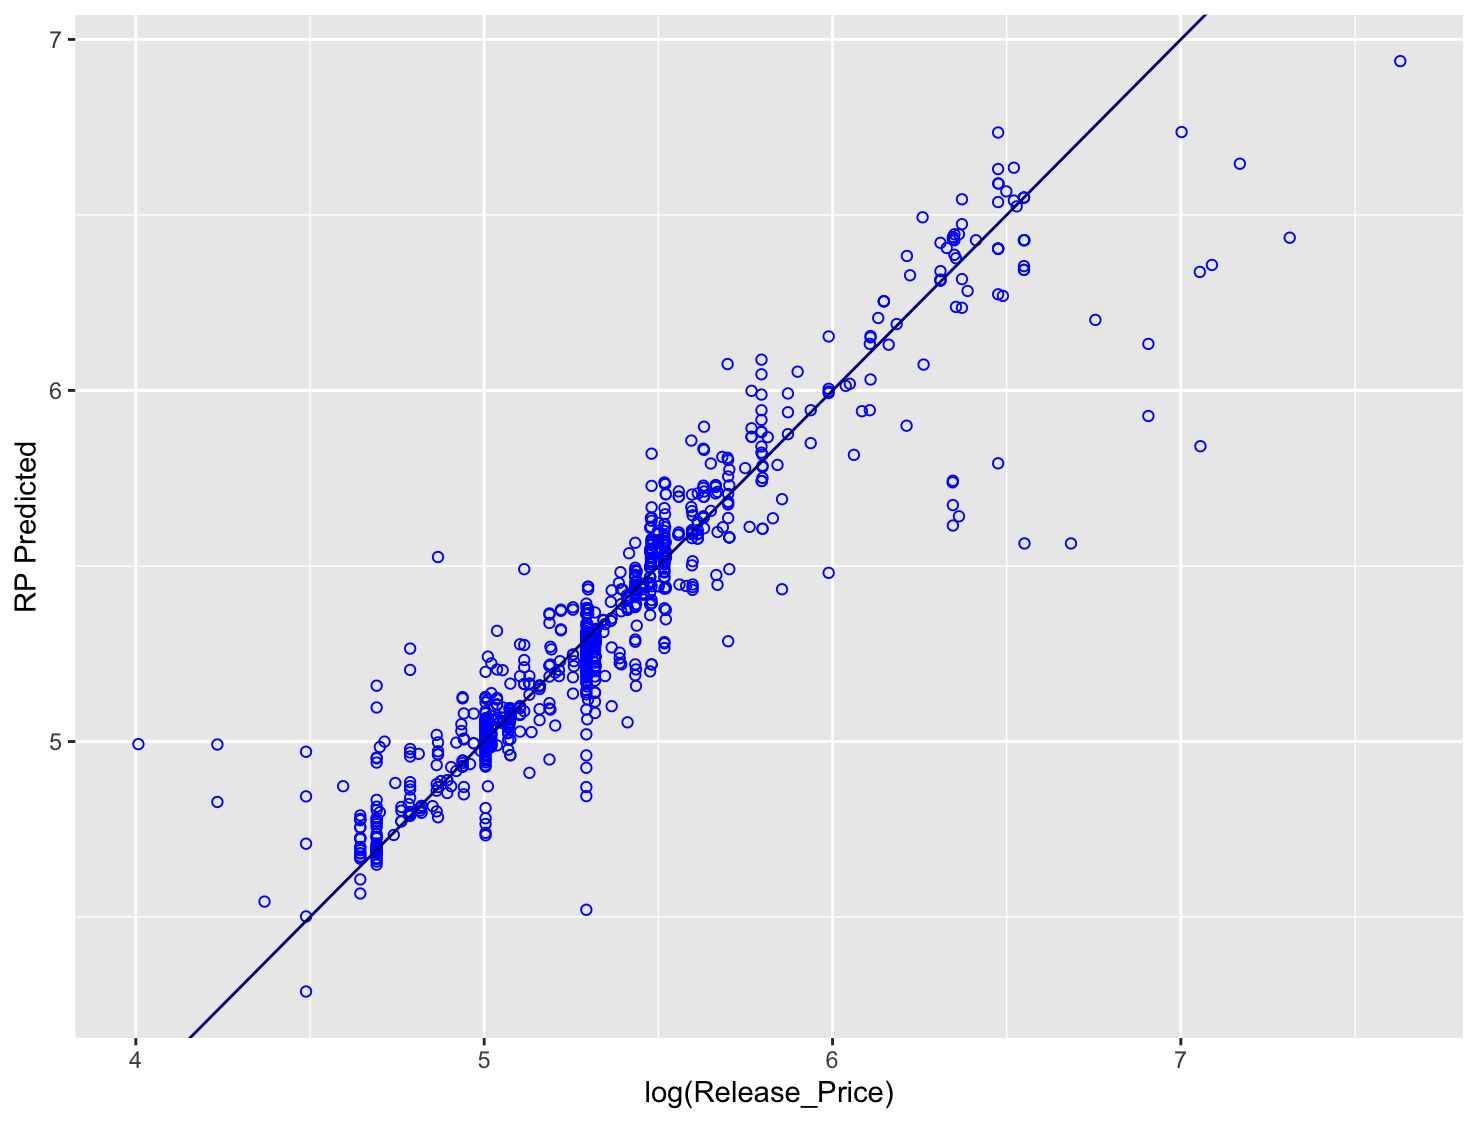
\includegraphics[width=8cm]{images/scatter_rfr.png}
\end{center}
\caption{Random Forest prediction plot}
\end{figure}
In comparison to other prediction plot, it is clear that the random forest prediction plot below has more points closer to the line than two other models, which means theoretically \textbf{Random Forest is the best model of all three}.
\pagebreak
\subsubsection{Comparison}
To determine between multi-linear regression, SVM regression and Random Forest Regression which one is more efficient exactly, we will consider the rate of accuracy of two models(calculated by subtracting SSE from SST, dividing the result by SST, and then multiplying by 100 to express the accuracy as a percentage).As can be seen above we have calculated and show the results of each model.
\begin{mdframed}[leftline=false,rightline=false,backgroundcolor=lightblue!10,nobreak=false]
    \begin{minted}[linenos,breaklines,breaksymbolleft=,obeytabs=true,tabsize=2]{R}
The accuracy of the model on test set: 56.73% #multi-linear
The accuracy of the model on test set: 83.72% #SVM 
The accuracy of the model on test set: 88.15% #Random Forest
\end{minted}
\end{mdframed}
Since \textbf{Random Forest} has a better accuracy rate, we should check their RMSE (Root Mean Squared Error) and MAE (Mean Absolute Error) for a better evaluation.

\begin{mdframed}[leftline=false,rightline=false,backgroundcolor=lightblue!10,nobreak=false]
    \begin{minted}[linenos,breaklines,breaksymbolleft=,obeytabs=true,tabsize=2]{R}
> paste("RMSE for model1: ", rmse_m1)
[1] "RMSE for model1:  0.301143401362998"
> paste("MAE for model1: ", mae_m1)
[1] "MAE for model1:  0.229336454060829"
> paste("RMSE for model2: ", rmse_m2)
[1] "RMSE for model2:  0.18474145956431"
> paste("MAE for model2: ", mae_m2)
[1] "MAE for model2:  0.108300786582277"
> paste("RMSE for model3: ", rmse_m3)
[1] "RMSE for model3:  0.157580846686117"
> paste("MAE for model3: ", mae_m3)
[1] "MAE for model3:  0.0834563933389319"
\end{minted}
\end{mdframed}
\textbf{Model3(Random Forest)} significantly outperforms the other two models on all three metrics. It has the lowest RMSE and MAE, meaning the model has the smallest average errors in predicting GPU prices. In conclusion, Random Forest regression has a better performance in GPU release\textunderscore price prediction than others.
\pagebreak
\section{Data and code availability}
\subsection{Dataset}
\href{https://www.kaggle.com/datasets/iliassekkaf/computerparts/data?select=All_GPUs.csv}{DATASET}
\subsection{Code}
\href{https://github.com/NhtJm/GR09-03}{CODE}
\section{Conclusion}
Throughout our project journey and the extensive process of compiling this comprehensive report, our team has traversed a multitude of significant milestones, demonstrating remarkable growth and proficiency in various domains:
\begin{itemize}
    \item \textbf{Data Mastery:}
    Our team has developed a robust understanding of data management, encompassing the nuanced art of handling data loss or corruption instances with finesse. Additionally, we have delved deep into the realm of statistical graphs, mastering their creation and interpretation to succinctly encapsulate and communicate our research findings.
    \item \textbf{R and RStudio Proficiency:}
    The intricate intricacies of R and RStudio have been thoroughly explored and harnessed to our advantage. This newfound proficiency has empowered us to embark on insightful data analyses, leveraging the extensive functionalities offered by these tools to derive meaningful insights from the datasets at hand. 
    \item \textbf{Bridging Theory with Practice:}
    A pivotal achievement for our team has been the successful transition from theoretical concepts gleaned within the confines of the classroom to their pragmatic application in real-world scenarios. This transition has been underpinned by our adept utilization of appropriate testing methodologies, ensuring the robustness and reliability of our research endeavors.
    \item \textbf{Continuous Learning and Adaptation:}
    Our journey has been characterized by an unwavering commitment to continuous learning and adaptation. We have not only embraced the acquisition of new knowledge but also seamlessly integrated it into our problem-solving repertoire. Despite encountering myriad obstacles along the way, such as navigating the intricacies of regression models for predictive analysis, we have demonstrated resilience and agility in overcoming these challenges.
    \item \textbf{Collaborative Excellence:}
    Collaboration lies at the heart of our team's success, as we have fostered a culture of mutual support and synergy. By leveraging each other's diverse skill sets and perspectives, we have synergistically worked towards our shared objectives, achieving remarkable outcomes that exceed the sum of our individual contributions.
\end{itemize}
In acknowledging the inherent limitations stemming from our individual capacities and knowledge bases, we humbly embrace the opportunity for improvement. Thus, we earnestly invite and welcome contributions and feedback from our peers and mentors, recognizing that constructive critique serves as a catalyst for growth and refinement. Your insights and suggestions are invaluable to us as we continue to strive for excellence in our academic and professional endeavors.
\pagebreak
\begin{thebibliography}{9}
    \bibitem{bib1} D. C. Montgomery and G. C. Runger, \emph{Applied Statistics and Probability for Engineers}, 7th ed. Kendallville: Wiley, 2018.
    \bibitem{bib2} T. D. Nguyen and D. H. Nguyen, \emph{Probability – Statistics and Data Analysis}. Ho Chi Minh City: VNUHCM Press, 2020.
    \bibitem{bib3} Zoumana Keita, \emph{Multiple Linear Regression in R: Tutorial With Examples}, Nov, 2022. [Online]. Available: \href{https://www.datacamp.com/tutorial/multiple-linear-regression-r-tutorial}{https://www.datacamp.com/tutorial/multiple-linear-regression-r-tutorial}.
    \bibitem{bib4} \emph{Random Forest Regression in Python Explained } [Online]\href{https://builtin.com/data-science/random-forest-python}{https://builtin.com/data-science/random-forest-python}.
    \bibitem{bib5} \emph{Usage of KNN }[Online]\href{https://www.ibm.com/docs/en/db2oc?topic=knn-usage}{https://www.ibm.com/docs/en/db2oc?topic=knn-usage}.
    \bibitem{bib6} \emph{Top Evaluation Metrics}[Online]\href{https://www.freecodecamp.org/news/evaluation-metrics-for-regression-problems-machine-learning/}{https://www.freecodecamp.org/news/evaluation-metrics-for-regression-problems-machine-learning/} 
    \bibitem{bib7} \emph{Log-Trans}
    [Online]\href{https://www.ncbi.nlm.nih.gov/pmc/articles/PMC4120293/}{https://www.ncbi.nlm.nih.gov/pmc/articles/PMC4120293/}
    \bibitem{bib8} K. Yang, J. Tu and T. Chen, \emph{Homoscedasticity: an overlooked critical assumption for linear regression}, 2019;32:e100148. doi: 10.1136/gpsych-2019-100148.
    \bibitem{bib9} P. Jonsson and C. Wohlin, “An evaluation of k-nearest neighbour imputation using Likert data,” \emph{10th International Symposium on Software Metrics, 2004. Proceedings.}, 2004, pp. 108-118, doi: 10.1109/METRIC.2004.1357895.
    \bibitem{bib10} Geeksforgeeks, \emph{Support Vector Machine (SVM) Algorithm}, [Online]. Available: \href{https://www.geeksforgeeks.org/support-vector-machine-algorithm/}{https://www.geeksforgeeks.org/support-vector-machine-algorithm/}.
    
\end{thebibliography}
\end{document}

